\subsection{\texorpdfstring{Characterization of measures with base \(\mu\)}{Characterization of measures with base mu}}

THEOREM 2 (Lebesgue--Nikodym). --- Let \(\mu\) and \(\nu\) be two positive measures on T. The following properties are equivalent:

\begin{enumerate}
\def\labelenumi{\arabic{enumi})}
\item
  \(\nu\) is a measure with base \(\mu\) .
\item
  Every locally \(\mu\) -negligible set is locally \(\nu\) -negligible.
\item
  Every \(\mu\) -negligible compact set is \(\nu\) -negligible.
\end{enumerate}

It is clear that 1) implies 2) (Cor. 1 of Prop. 3), and that 2) implies 3). We are going to show that 3) implies 1). We first note that if the condition 3) is satisfied, then every set A that is universally measurable and locally \(\mu\) -negligible is locally \(\nu\) -negligible; for, \(\nu^{\bullet}(\mathrm{A}) = \sup \nu(\mathrm{K})\) , where K runs over the set of compact sets contained in A ( \(\S 1\) , No.~3, Prop. 10, a) and Ch. IV, \(\S 4\) , No.~6, Cor. 2 of Th. 4). Next, we shall establish two lemmas.

Lemma 2. --- Let \(\alpha\) be a bounded positive measure on T, and \(\beta\) a real measure on T such that \(|\beta| \leqslant M\alpha\) , where M is a positive constant. Then, there exists a real function \(u\) , \(\alpha\) -integrable, such that \(\beta = u \cdot \alpha\) .

Let \(g\) be an element of the space \(\mathcal{L}_{\mathbf{R}}^{2}(\mathrm{T},\alpha)\) ; \(g\) is \(\beta\) -measurable and \(\int^{\bullet}|g|^2 d|\beta| \leqslant \mathrm{M}\int^{\bullet}|g|^2 d\alpha < +\infty\) . The function \(g\) therefore belongs to \(\mathcal{L}^2 (\mathrm{T},|\beta|)\) , and also to \(\mathcal{L}^1 (\mathrm{T},|\beta|)\) since \(\beta\) is bounded. By the Cauchy-Schwarz inequality,

\[
| \beta (g) | ^ {2} \leqslant \left(\int | g | d | \beta |\right) ^ {2} \leqslant \left(\int d | \beta |\right) \left(\int | g | ^ {2} d | \beta |\right) \leqslant \mathrm{M} ^ {2} \alpha (1) \alpha (| g | ^ {2}).
\]

The mapping \(g \mapsto \beta(g)\) is thus a continuous linear form on \(\mathcal{L}^2(\mathrm{T},\alpha)\) . The Hausdorff space associated with \(\mathcal{L}^2(\mathrm{T},\alpha)\) being a Hilbert space, there then exists (TVS, Ch. V, §1, No.~7, Th. 3) a real function \(u \in \mathcal{L}^2(\mathrm{T},\alpha)\) , therefore also belonging to \(\mathcal{L}^1(\mathrm{T},\alpha)\) , such that \(\beta(g) = \alpha(ug)\) for every \(g \in \mathcal{L}^2(\mathrm{T},\alpha)\) . Applying this relation for \(g \in \mathcal{K}(\mathrm{T})\) , one sees that \(\beta = u\cdot \alpha\) .

Lemma 3. --- Suppose that the positive measure \(\nu\) is such that every \(\mu\) -negligible compact set is \(\nu\) -negligible. Let \(\mathfrak{K}\) be the set of compact subsets \(K\) of \(T\) having the following property:

\begin{enumerate}
\def\labelenumi{(\arabic{enumi})}
\setcounter{enumi}{10}
\tightlist
\item
  There exists a constant \(M \geqslant 0\) such that \(\varphi_{K} \cdot \nu \leqslant M \varphi_{K} \cdot \mu\) . The set K is then \(\mu\) -dense in T.
\end{enumerate}

If K satisfies (11), and if A is a Borel set contained in K, it follows at once from Prop. 8 that \(\varphi_{\mathrm{A}} \cdot \nu \leqslant \mathrm{M}\varphi_{\mathrm{A}} \cdot \mu\) ; from this, one deduces that the union of two elements K, \(K'\) of \(\mathfrak{K}\) belongs to \(\mathfrak{K}\) because \(\varphi_{\mathrm{K} \cup \mathrm{K}'} = \varphi_{\mathrm{K}} + \varphi_{\mathrm{A}}\) , where \(\mathrm{A} = \mathrm{K}' \cap \mathbb{C}\mathrm{K}\) . To establish the lemma, it remains to prove that every compact set L such that \(\mu(\mathrm{L}) > 0\) contains a compact set \(\mathrm{K} \in \mathfrak{K}\) such that \(\mu(\mathrm{K}) > 0\) (Ch. IV, §5, No.~8, Prop. 12). Choose a number \(\mathrm{M} > \nu(\mathrm{L}) / \mu(\mathrm{L})\) and apply Lemma 1 to the bounded positive measure \(\alpha = \varphi_{\mathrm{L}} \cdot (\nu + \mathrm{M}\mu)\) and the measure \(\beta = \varphi_{\mathrm{L}} \cdot (\nu - \mathrm{M}\mu)\) . Replacing if necessary the function \(u\) such that \(\beta = u \cdot \alpha\) by a function equal to it \(\alpha\) -almost everywhere, one can suppose that \(u\) is universally measurable (§3, No.~4, Prop. 7) and is zero outside of L. The set H of \(t \in \mathrm{T}\) such that \(u(t) < 0\) , which is contained in L, could not be \(\mu\) -negligible, for it would then be \(\nu\) -negligible (by the remark made at the beginning of the proof of Th. 2), hence \(\alpha\) -negligible, and one would have \(\beta(\mathrm{L}) > 0\) , which contradicts the choice of M. Let K be a compact set contained in H, such that \(\mu(\mathrm{K}) > 0\) ; let us show that \(\mathrm{K} \in \mathfrak{K}\) , which will establish the lemma. By Prop. 8,

\[
\varphi_ {\mathrm{K}} \cdot (\nu - \mathrm{M} \mu) = \varphi_ {\mathrm{K}} \cdot \beta = \varphi_ {\mathrm{K}} \cdot (u \cdot \alpha) = (\varphi_ {\mathrm{K}} u) \cdot \alpha .
\]

The function \(\varphi_{\mathbf{K}}u\) is negative, therefore we indeed have \(\varphi_{\mathbf{K}}\cdot \nu \leqslant \mathrm{M}\varphi_{\mathbf{K}}\cdot \mu\) .

Let us now complete the proof of Theorem 2. Assume that the condition 3) is verified and define \(\mathfrak{K}\) as in Lemma 3. Let \((\mathrm{K}_{\alpha})_{\alpha \in \mathbf{A}}\) be a locally countable family of pairwise disjoint elements of \(\mathfrak{K}\) , such that the set \(\mathrm{N} = \mathrm{T} - \bigcup_{\alpha \in \mathbf{A}} \mathrm{K}_{\alpha}\) is locally \(\mu\) -negligible (Ch. IV, §5, No.~9, Prop. 14); the family \((\mathrm{K}_{\alpha})\) being locally countable, N is universally measurable and therefore locally \(\nu\) -negligible. Set \(\mu_{\alpha} = \varphi_{\mathrm{K}_{\alpha}} \cdot \mu\) , \(\nu_{\alpha} = \varphi_{\mathrm{K}_{\alpha}} \cdot \nu\) ; since the functions \(\varphi_{\mathrm{K}_{\alpha}}\) form a locally countable family, whose sum is equal to 1 locally almost everywhere for \(\mu\) and for \(\nu\) , Proposition 6 implies that \(\mu = \sum_{\alpha \in \mathbf{A}} \mu_{\alpha}\) , \(\nu = \sum_{\alpha \in \mathbf{A}} \nu_{\alpha}\) . On the other hand, by the definition of \(\mathfrak{K}\) , there exists for every \(\alpha\) a constant \(\mathrm{M}_{\alpha}\) such that \(\nu_{\alpha} \leqslant \mathrm{M}_{\alpha} \mu_{\alpha}\) ; Lemma 2 therefore implies the existence of a function \(g_{\alpha}\) , which one can suppose to be zero outside of \(\mathrm{K}_{\alpha}\) and positive (Cor. 3 of Prop. 3), such that \(\nu_{\alpha} = g_{\alpha} \cdot \mu_{\alpha}\) . Therefore (No.~4, Prop. 8)

\[
\nu_ {\alpha} = g _ {\alpha} \cdot \mu_ {\alpha} = g _ {\alpha} \cdot (\varphi_ {\mathrm{K} _ {\alpha}} \cdot \mu) = (g _ {\alpha} \varphi_ {\mathrm{K} _ {\alpha}}) \cdot \mu = g _ {\alpha} \cdot \mu .
\]

Set \(g = \sum_{\alpha \in A} g_{\alpha}\) ; since the family \((g_{\alpha})\) is locally countable and the family \((\nu_{\alpha})\) is summable, Proposition 6 implies that \(g\) is locally \(\mu\) -integrable, and that \(\nu = g \cdot \mu\) , which establishes the theorem.

COROLLARY 1. --- Let N be a set of positive measures with base \(\mu\) , admitting a supremum \(\nu\) in \(\mathcal{M}(\mathrm{T})\) ; then \(\nu\) is a measure with base \(\mu\) .

The Cor. of Prop. 2 permits reduction to the case that N is an increasing directed set. For every locally \(\mu\) -negligible set A one then has, by Prop. 11 of §1, No.~4,

\[
\nu^ {\bullet} (\mathrm{A}) = \sup _ {\lambda \in \mathcal {N}} \lambda^ {\bullet} (\mathrm{A}) = 0.
\]

Theorem 2 therefore implies that \(\nu\) is a measure with base \(\mu\) .

COROLLARY 2. --- Let \(\nu\) be a real measure on T. In order that \(\nu\) belong to the band generated by \(\mu\) in the fully lattice-ordered space \(\mathcal{M}(\mathrm{T})\) (Ch. II, §1, No.~5), it is necessary and sufficient that \(\nu\) be a measure with base \(\mu\) .

On considering \(\nu^{+}\) and \(\nu^{-}\) , one is immediately reduced to the case of a positive measure \(\nu\) (No.~2, Cor. of Prop. 2). Let us then set \(\nu_{n} = \inf(n\mu, \nu)\) ; \(\nu\) belongs to the band generated by \(\mu\) if and only if \(\nu = \sup_{n} \nu_{n}\) (Ch. II, §1,

No.~5, Cor. of Prop. 6). Now \(\nu_{n}\) , being bounded above by \(n\mu\) , is a measure with base \(\mu\) by Th. 2; the relation \(\nu = \sup_{n} \nu_{n}\) therefore implies that \(\nu\) is

a measure with base \(\mu\) (Cor. 1). Conversely, suppose that \(\nu\) is a measure with base \(\mu\) : \(\nu = g \cdot \mu\) , where \(g\) is locally \(\mu\) -integrable and positive. Then \(\nu_n = \inf(g, n) \cdot \mu\) (Cor. of Prop. 2), and it follows at once from Lebesgue's theorem (Ch. IV, §4, No.~3, Prop. 4) that \(\nu = \sup_{n} \nu_n\) .

COROLLARY 3. --- Let \(\theta\) be a complex measure; there exists a universally measurable function \(v\) , with \(|v| = 1\) , such that \(\theta = v \cdot |\theta|\) , \(|\theta| = \overline{v} \cdot \theta\) .

Write \(\theta = \theta_{1} - \theta_{2} + i(\theta_{3} - \theta_{4})\) , where \(\theta_{1} = (\mathcal{R}\theta)^{+}\) , \(\theta_{2} = (\mathcal{R}\theta)^{-}\) , \(\theta_{3} = (\mathcal{I}\theta)^{+}\) , \(\theta_{4} = (\mathcal{I}\theta)^{-}\) ; the positive measures \(\theta_{i} (i = 1, 2, 3, 4)\) , being bounded above by \(|\theta|\) (Ch. III, §1, No.~6, formula (17)), are measures with base \(|\theta|\) by Theorem 2. It follows that there exists a locally \(|\theta|\) -integrable function v such that \(\theta = v \cdot |\theta|\) . Proposition 2 then yields the relation \(|\theta| = |v| \cdot |\theta|\) , which implies that \(|v| = 1\) locally \(|\theta|\) -almost everywhere (Cor. 2 of Prop. 3). Finally, by Prop. 8, \(\overline{v} \cdot \theta = (v\overline{v}) \cdot |\theta| = |\theta|\) . Since the function v is defined only up to a locally \(|\theta|\) -negligible function, one can suppose that v is universally measurable (§3, No.~4, Prop. 7) and that \(|v| = 1\) everywhere.

Remarks. --- 1) Suppose that \(\lambda\) is a positive measure, that \(v\) is a \(\lambda\) -measurable function such that \(|v| = 1\) locally \(\lambda\) -almost everywhere (which implies that \(v\) is locally \(\lambda\) -integrable), and that \(\theta = v \cdot \lambda\) . Prop. 2 shows immediately that \(\lambda = |\theta|\) ; in other words, the property of the preceding statement characterizes the positive measure \(|\theta|\) .

\begin{enumerate}
\def\labelenumi{\arabic{enumi})}
\setcounter{enumi}{1}
\tightlist
\item
  If \(|\theta| \leqslant a\mu\) , where \(\mu\) is a positive measure and \(a\) is a number \(\geqslant 0\) , then \(\theta\) is a measure with base \(\mu\) .
\end{enumerate}

COROLLARY 4. --- Let \(\rho\) and \(\theta\) be two complex measures. In order that there exist a locally \(\theta\) -integrable function \(u\) such that \(\rho = u \cdot \theta\) , it is necessary and sufficient that every \(\theta\) -negligible compact set be \(\rho\) -negligible.

The condition is obviously necessary. Conversely, suppose that every \(\theta\) -negligible compact set is \(\rho\) -negligible; Theorem 2 implies the existence of a locally \(|\theta|\) -integrable function g such that \(|\rho| = g \cdot |\theta|\) . On the other hand, Cor. 3 implies the existence of a function \(v_{1}\) (resp. \(v_{2}\) ), of absolute value 1 and measurable for the measure \(|\rho|\) (resp. \(\theta\) ), such that \(\rho = v_{1} \cdot |\rho|\) (resp. \(|\theta| = \overline{v}_{2} \cdot \theta\) ). Then, by Prop. 8, \(\rho = u \cdot \theta\) with \(u = v_{1}g\overline{v}_{2}\) .

COROLLARY 5. --- Let \(\mu\) and \(\nu\) be two positive measures on T. The conditions 1), 2), 3) of Th. 2 are also equivalent to the following ones:

\begin{enumerate}
\def\labelenumi{\arabic{enumi})}
\setcounter{enumi}{3}
\item
  For every \(\nu\) -integrable numerical function \(f \geqslant 0\) and for every number \(\varepsilon > 0\) , there exists a \(\delta > 0\) such that the relations \(0 \leqslant h \leqslant f\) and \(\int^{*} h d\mu \leqslant \delta\) imply \(\int^{*} h d\nu < \varepsilon\) .
\item
  For every function \(g \in \mathcal{K}_{+}(\mathrm{T})\) and every number \(\varepsilon > 0\) , there exists a \(\delta > 0\) such that, for every \(h \in \mathcal{K}_{+}(\mathrm{T})\) bounded above by \(g\) and satisfying \(\int h d\mu \leqslant \delta\) , one has \(\int h d\nu \leqslant \varepsilon\) .
\item
  For every compact set \(\mathbf{K} \subset \mathbf{T}\) and every number \(\varepsilon > 0\) , there exists a \(\delta > 0\) such that the relations \(\mathbf{A} \subset \mathbf{K}\) and \(\mu^{*}(\mathbf{A}) \leqslant \delta\) imply \(\nu^{*}(\mathbf{A}) \leqslant \varepsilon\) . The implications 4) \(\Rightarrow 6) \Rightarrow 3)\) are obvious.
\end{enumerate}

Suppose there exists a finite function \(k \geqslant 0\) , universally measurable and locally \(\mu\) -integrable, such that \(\nu = k \cdot \mu\) , and let us show that the condition 4) is satisfied. Let f be a \(\nu\) -integrable function \(\geqslant 0\) , and let \(\varepsilon > 0\) . For every integer \(n \geqslant 0\) , let \(A_{n}\) be the set of \(t \in T\) such that \(k(t) \geqslant n\) . The functions \(f\varphi_{A_{n}}\) form a decreasing sequence, bounded above by f and tending pointwise to 0, therefore there exists an N such that \(\int f\varphi_{A_{N}} d\nu \leqslant \varepsilon/2\) (Ch. IV, §4, No.~3, Prop. 4). If h is a function on T satisfying \(0 \leqslant h \leqslant f\) and \(\int^{*} h d\mu \leqslant \varepsilon/2N\) , then

\[
\begin{array}{r l} & {\nu^ {*} (h) \leqslant \nu^ {*} (h \varphi_ {\mathrm {A_ {N}}}) + \nu^ {*} \big (h (1 - \varphi_ {\mathrm {A_ {N}}}) \big)} \\ & {\quad \leqslant \nu^ {*} (f \varphi_ {\mathrm {A_ {N}}}) + \mu^ {*} \big (h (1 - \varphi_ {\mathrm {A_ {N}}}) k \big)} \\ & {\quad \leqslant \frac {\varepsilon}{2} + \mathrm{N} \mu^ {*} (h) \leqslant \varepsilon .} \end{array}
\]

We have thus proved that the conditions 4) and 6) are equivalent to the conditions of Th. 2.

It is clear that 4) implies 5). Finally, if the condition 5) is satisfied, then \(\nu\) belongs to the band generated by \(\mu\) (Ch. II, §2, No.~2, Prop. 5), hence has base \(\mu\) (Cor. 2).

Scholium. --- For every \(\dot{f} \in \mathrm{L}_{\mathrm{loc}}^{1}(\mathrm{T}, \mu; \mathbf{R})\) , set \(\varphi(\dot{f}) = f \cdot \mu\) , where \(f \in \dot{f}\) ; the mapping \(\varphi\) is linear, increasing and injective (Cor. 2 of Prop. 3), and its image in \(\mathcal{M}(\mathrm{T})\) is the band B generated by \(\mu\) (Cor. 2 of Th. 2). The mapping \(\varphi\) therefore permits identifying \(\mathrm{L}_{\mathrm{loc}}^{1}(\mathrm{T},\mu;\mathbf{R})\) with a space of real measures on T; since all of the spaces \(\mathrm{L}_{\mathbf{R}}^{p}(\mathrm{T},\mu)\) are subspaces of \(\mathrm{L}_{\mathrm{loc}}^{1}(\mathrm{T},\mu;\mathbf{R})\) , they too may be identified with subspaces of \(\mathcal{M}(\mathrm{T})\) . Analogous considerations hold for complex-valued functions and measures. Note that the mapping \(\varphi\) considered above is an isomorphism of the ordered vector space structures of \(L_{loc}^{1}\) and B, but is obviously not an isomorphism for the topological vector space structures of these spaces.

\pandocbounded{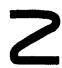
\includegraphics[keepaspectratio]{images/part002_ab1a0807.jpg}}

Since every band in a fully lattice-ordered space is itself a fully lattice-ordered space (Ch. II, §1, No.~5), one sees that the space \(L_{loc}^{1}\) is fully lattice-ordered; but it is worthwhile to recall that the supremum in \(L_{loc}^{1}\) of an uncountable family \((\dot{f}_{\alpha})\) of equivalence classes is not necessarily identical to the class of the upper envelope of the functions \(f_{\alpha}\) . However, we saw that for an increasing sequence \((f_{n})\) of locally \(\mu\) -integrable functions whose upper envelope f is locally \(\mu\) -integrable, \(f \cdot \mu\) is the supremum of the sequence of measures \((f_{n} \cdot \mu)\) in \(\mathcal{M}(T)\) (Cor. of Prop. 6).

Here is an interesting consequence of Corollary 3 of Th. 2:

PROPOSITION 9. --- Let \(\theta\) be a bounded complex measure; for \(\theta\) to be a positive measure, it is necessary and sufficient that \(\| \theta \| = \theta(1)\) .

The condition is obviously necessary. Conversely, suppose that \(\|\theta\|=\int d\theta\) , and denote by v a \(|\theta|\) -measurable function of absolute value 1 such that \(\theta=v\cdot|\theta|\) . Since \(\|\theta\|=\int d|\theta|\) (Ch. IV, §4, No.~7, Prop. 12) and \(\int d\theta=\int v\cdot d|\theta|\) (Th. 1), the hypothesis implies that \(\int(1-v)d|\theta|=0\) and therefore \(\int\mathcal{R}(1-v)d|\theta|=0\) . The function \(\mathcal{R}(1-v)\) , being positive, is therefore zero almost everywhere, which implies that v=1 almost everywhere and completes the proof.

\subsection{Equivalent measures}

PROPOSITION 10. --- Let \(\mu\) and \(\nu\) be two positive measures on T. The following conditions are equivalent:

\begin{enumerate}
\def\labelenumi{\alph{enumi})}
\item
  The locally negligible sets are the same for \(\mu\) and \(\nu\) .
\item
  The bands generated by \(\mu\) and \(\nu\) in \(\mathcal{M}(\mathrm{T})\) are identical.
\item
  One has \(\nu = g \cdot \mu\) , where \(g\) is locally \(\mu\) -integrable and \(g(t) > 0\) locally almost everywhere for \(\mu\) .
\end{enumerate}

The conditions a) and b) are equivalent by Cor. 2 of Th. 2 of No.~5. If they are satisfied, then \(\nu = g \cdot \mu\) and \(\mu = h \cdot \nu\) , where \(g\) (resp. \(h\) ) is positive and locally integrable for \(\mu\) (resp. \(\nu\) ). Therefore (No.~4, Prop. 8) \(hg\) is locally \(\mu\) -integrable and \(\mu = (hg) \cdot \mu\) . It follows (No.~3, Cor. 2 of Prop. 3) that \(hg\) is equal to 1 locally almost everywhere for \(\mu\) , so that \(g(t) > 0\) and \(h(t) = 1/g(t)\) locally almost everywhere for \(\mu\) . Conversely, suppose that \(\nu = g \cdot \mu\) with \(g(t) > 0\) locally almost everywhere for \(\mu\) ;

since \((1/g)g\) is defined locally almost everywhere and is locally \(\mu\) -integrable, 1/g is locally \(\nu\) -integrable and \((1/g)\cdot\nu=\mu\) (No.~4, Prop. 8).

DEFINITION 3. --- Two complex measures \(\theta, \theta'\) on a locally compact space T are said to be equivalent if the measures \(|\theta|\) and \(|\theta'|\) satisfy the conditions a), b), c) of Prop. 10.

For \(\theta\) and \(\theta'\) to be equivalent, it is therefore necessary and sufficient that \(|\theta|\) and \(|\theta'|\) be equivalent.

Remark. --- If \(\mu\) and \(\nu\) are two equivalent positive measures then the measurable functions defined on T, with values in any topological space G, are the same for \(\mu\) and \(\nu\) , as follows at once from Prop. 4 of No.~3.

PROPOSITION 11. --- Let \(\mu\) be a positive measure on T. If T is countable at infinity, then there exists a continuous function \(h\) such that \(h(t) > 0\) for all \(t \in \mathrm{T}\) and such that the measure \(\nu = h \cdot \mu\) (equivalent to \(\mu\) ) is bounded.

Let \((\mathrm{K}_{n})\) be a sequence of compact sets forming a covering of T and, for every n, let \(f_{n}\) be a function in \(\mathcal{K}(\mathrm{T})\) such that \(0 \leqslant f_{n} \leqslant 1\) and \(f_{n}(t) = 1\) on \(\mathrm{K}_{n}\) (Ch. III, §1, No.~2, Lemma 1). Let \((a_{n})\) be a sequence of numbers \textgreater{} 0 such that \(\sum_{n} a_{n} < +\infty\) ; the series \(h = \sum_{n} a_{n} f_{n}\) is then normally convergent in T, consequently h is a continuous function on T, such that \(h(t) > 0\) for all \(t \in \mathrm{T}\) , by construction. Setting \(\nu = h \cdot \mu\) , we then have (Prop. 3 and Ch. IV, §1, No.~3, Prop. 13)

\[
\nu^ {*} (1) = \int^ {*} h d \mu \leqslant \sum_ {n} a _ {n} \int f _ {n} d \mu .
\]

On taking for example \(a_{n} = 2^{-n}\left(\int f_{n}d\mu\right)^{-1}\) when \(\int f_n d\mu > 1\) , and \(a_{n} = 2^{-n}\) otherwise, we have \(\sum_{n}a_{n} < +\infty\) and \(\nu^{*}(1) < +\infty\) , which proves the proposition.

PROPOSITION 12. --- Let \((\mu_n)\) be a sequence of bounded positive measures on T; there exists a bounded positive measure \(\mu\) on T such that the relation \(\mu^*(\mathrm{N}) = 0\) is equivalent to \(\langle \mu_n^*(\mathrm{N}) = 0 \text{ for every } n \rangle\) ; each of the measures \(\mu_n\) has base \(\mu\) . Moreover, if \(\mu'\) is a second positive measure on T having this property, then \(\mu\) and \(\mu'\) are equivalent.

The last part of the statement follows at once from Def. 3. To prove the existence of \(\mu\) , we can restrict ourselves to the case that \(\mu_n \neq 0\) for every \(n\) ; the family of measures \(\mu_n / 2^n \| \mu_n \|\) is then summable in \(\mathcal{M}(\mathrm{T})\) , and its sum \(\mu\) is such that \(\| \mu \| \leqslant 1\) . Moreover, since \(\mu_n \leqslant 2^n \| \mu_n \| \cdot \mu\) , the relation \(\mu(\mathrm{N}) = 0\) implies that \(\mu_n(\mathrm{N}) = 0\) for all \(n\) ; conversely, if \(\mathrm{N}\) is a set that is negligible for all the \(\mu_n\) , then it is locally negligible for \(\mu\) (§2, No.~2, Cor. 2 of Prop. 1), hence is \(\mu\) -negligible since \(\mu\) is bounded (§1, No.~2, Cor. 2 of Prop. 7).

\subsection{Alien measures}

Given two real measures \(\rho,\sigma\) on T, recall that \(\rho\) and \(\sigma\) are said to be alien (to each other) if \(\inf(|\rho|,|\sigma|)=0\) in \(\mathcal{M}(\mathrm{T})\) (Ch. II, §1, No.~1). The real measures alien to a given measure are known to form a band (Ch. II, §1, No.~5, Th. 1). This definition may be extended immediately to the case of complex measures.

DEFINITION 4. --- One says that a complex measure \(\theta\) on T is concentrated on a subset M of T, or that M carries \(\theta\) , if \(\mathbb{C}M\) is locally negligible for \(\theta\) .

The set M carries \(\theta\) if and only if it carries \(|\theta|\) . It is equivalent to say that M carries \(\theta\) , or that M is \(\theta\) -measurable and \(\theta = \varphi_{M} \cdot \theta\) . If \(\theta\) is concentrated on M, then every measure with base \(|\theta|\) is concentrated on M.

PROPOSITION 13. --- In order that two complex measures \(\rho\) and \(\sigma\) on T be alien to each other, it is necessary and sufficient that there exist in T two disjoint sets R and S such that \(\rho\) is concentrated on R and \(\sigma\) on S; R and S may be taken to be universally measurable.

Set \(\mu = |\rho|\) , \(\nu = |\sigma|\) , \(\lambda = \mu + \nu\) ; since \(\mu\) and \(\nu\) are bounded above by \(\lambda\) , there exist two locally \(\lambda\) -integrable functions u and v (which one can suppose to be universally measurable by §3, No.~4, Prop. 7) such that \(\mu = u \cdot \lambda\) , \(\nu = v \cdot \lambda\) . Then

\[
\inf (| \rho |, | \sigma |) = \inf (\mu , \nu) = \inf (u, v) \cdot \lambda
\]

(No.~2, Cor. of Prop. 2). Let A (resp. B) be the set of \(t \in \mathbf{T}\) such that \(u(t) > 0\) and \(v(t) = 0\) (resp. \(u(t) = 0\) and \(v(t) > 0\) ). If \(\rho\) and \(\sigma\) are alien, then \(\inf(u, v) = 0\) locally \(\lambda\) -almost everywhere (No.~3, Cor. 2 of Prop. 3), so that the disjoint universally measurable sets A and B carry \(\mu\) and \(\nu\) , respectively. Conversely, suppose that \(\mu\) and \(\nu\) are carried, respectively, by disjoint sets R and S; \(\varphi_{\mathrm{R}}\) is measurable for the measure \(\mu = u \cdot \lambda\) , and \(\mu = \varphi_{\mathrm{R}} \cdot \mu\) . By Prop. 8 of No.~4, the function \(u' = u\varphi_{\mathrm{R}}\) is \(\lambda\) -measurable, and \(\mu = u' \cdot \lambda\) . Similarly, if \(v' = v\varphi_{\mathrm{S}}\) then \(\nu = v' \cdot \lambda\) ; one concludes by remarking that \(\inf(u', v') = 0\) (No.~2, Cor. of Prop. 2).

COROLLARY 1. --- For every real measure \(\nu\) on T, there exist two disjoint sets M,N carrying \(\nu^{+}\) and \(\nu^{-}\) , respectively.

\pandocbounded{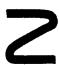
\includegraphics[keepaspectratio]{images/part002_61ad429f.jpg}}

One must take care not to confuse the notion of support of a measure \(\nu\) , and that of a set where \(\nu\) is concentrated. The support S of \(\nu\) is the smallest closed set carrying \(\nu\) (Ch. III, §2, No.~2, Prop. 2 and Ch. IV, §2, No.~2, Prop. 5). However, there may exist subsets of S that are distinct from S and carry \(\nu\) . More generally, one can have \(\inf(\mu,\nu)=0\) for two positive measures \(\mu\) and \(\nu\) having the same support (Exer. 5).

Note also that the intersection of the sets carrying \(\nu\) is the set of points \(t \in T\) such that \(|\nu|(\{t\}) > 0\) , and it can be empty (for example, in the case of Lebesgue measure); therefore, there is not in general a smallest set carrying \(\nu\) .

COROLLARY 2. --- Let \(\rho\) and \(\sigma\) be two alien complex measures, and let \(\rho'\) and \(\sigma'\) be two complex measures admitting densities relative to \(\rho\) and \(\sigma\) , respectively; then \(\rho'\) and \(\sigma'\) are alien.

COROLLARY 3. --- Let \(\rho\) and \(\sigma\) be two alien complex measures; then \(|\rho + \sigma| = |\rho| + |\sigma|\) .

Denote by v (resp. w) a universally measurable function of absolute value 1 such that \(\rho = v \cdot |\rho|\) (resp. \(\sigma = w \cdot |\sigma|\) ) (Cor. 3 of Th. 2), and by A a universally measurable set carrying \(\rho\) , such that B = C A carries \(\sigma\) (Prop. 13); then also \(\rho + \sigma = (v\varphi_{\mathrm{A}} + w\varphi_{\mathrm{B}}) \cdot (|\rho| + |\sigma|)\) . Since the function \(v\varphi_{A} + w\varphi_{B}\) has absolute value equal to 1, the corollary follows from Prop. 2.

THEOREM 3 (Lebesgue). --- Every complex measure \(\theta\) on T may be written in one and only one way in the form \(\theta = g \cdot \mu + \theta'\) , where \(g\) is locally \(\mu\) -integrable and \(\theta'\) is a measure alien to \(\mu\) . Then \(|\theta| = |g| \cdot \mu + |\theta'|\) .

When \(\theta\) is positive, this follows at once from the theorem of F. Riesz (Ch. II, §1, No.~5, Th. 1) applied to the fully lattice-ordered space \(\mathcal{M}(T)\) of real measures on T, and to the band generated by \(\mu\) in this space, on taking into account Cor. 2 of No.~5, Th. 2; moreover, \(\theta'\) and \(g \cdot \mu\) are then positive, which implies that \(g\) is positive locally \(\mu\) -almost everywhere (Cor. 3 of Prop. 3). To treat the case that \(\theta\) is not positive, set \(\nu = |\theta|\) , \(\nu = f \cdot \mu + \nu'\) (where \(f\) is positive and where \(\nu'\) and \(\mu\) are alien to each other), and \(\theta = v \cdot \nu\) , where \(v\) is a universally measurable function of absolute value 1 (Cor. 3 of Th. 2). We then have (Prop. 8) \(\theta = g \cdot \mu + \theta'\) , with \(g = vf\) (so that \(|g| = f\) ) and \(\theta' = v \cdot \nu'\) (so that \(|\theta'| = \nu'\) by Prop. 2); the measures \(\theta'\) and \(\mu\) are alien to each other by Cor. 2 of Prop. 13. It only remains to establish the uniqueness of the decomposition. Thus, suppose that \(\theta = g \cdot \mu + \theta' = g_1 \cdot \mu + \theta'_1\) , where \(\theta'\) and \(\theta'_1\) are alien to \(\mu\) ; \(|\theta' - \theta'_1|\) is bounded above by \(|\theta'| + |\theta'_1|\) , therefore \(\theta' - \theta'_1\) is alien to \(\mu\) , hence also to \((g_1 - g) \cdot \mu\) . The relation \(\theta' - \theta'_1 = (g_1 - g) \cdot \mu\) then implies that the two members are zero, which proves uniqueness.

Recall (No.~5, Th. 2 and Scholium) that the space \(\mathrm{L}_{\mathrm{loc}}^{1}(\mathrm{T},\mu;\mathbf{C})\) may be identified (by means of the mapping \(g\mapsto g\cdot\mu\) ) with a subspace of \(\mathcal{M}_{\mathbf{C}}(\mathrm{T})\) . With this convention, Theorem 3 takes the following form:

COROLLARY. --- There exists a projector \(p\) of the space \(\mathcal{M}_{\mathbf{C}}(\mathrm{T})\) onto the space \(\mathrm{L}_{\mathrm{loc}}^{1}(\mathrm{T},\mu ;\mathbf{C})\) , whose kernel \(\overline{p}^{1}(0)\) is the set of complex measures alien to \(\mu\) , such that

\[
| \theta | = | p (\theta) | + | \theta - p (\theta) |, \quad p (| \theta |) = | p (\theta) |
\]

for every complex measure \(\theta\) .

If p is restricted to the set of bounded measures, one obtains a projector \(p^{1}\) of the space \(\mathcal{M}_{\mathbf{C}}^{1}(\mathrm{T})\) onto the space \(\mathrm{L}_{\mathbf{C}}^{1}(\mathrm{T},\mu)\) ; the relation \(\|\theta\|=|\theta|(1)\) implies that \(\|\theta\|=\|p^{1}(\theta)\|+\|\theta-p^{1}(\theta)\|\) for every bounded complex measure \(\theta\) .

\subsection{\texorpdfstring{Applications: I. Duality of the spaces \(L^{p}\)}{Applications: I. Duality of the spaces L to the p}}

We shall treat here only the case of the real spaces \(\mathbf{L}^p\) .

Recall that two numbers \(p, q\) such that \(1 \leqslant p \leqslant +\infty\) , \(1 \leqslant q \leqslant +\infty\) , \(1/p + 1/q = 1\) are said to be conjugate exponents (Ch. IV, §6, No.~4). Every function \(g \in \mathcal{L}^q\) defines a continuous linear form \(\theta_g\) on \(L to the p\) , obtained by passing to the quotient starting with the linear form \(f \mapsto \int fg d\mu\) on \(\mathcal{L}^p\) , and one has \(N_q(g) = \| \theta_g \|\) (Ch. IV, §6, No.~4, Cor. of Prop. 3). Passing to the quotient, one thus deduces from the mapping \(g \mapsto \theta_g\) an isometric linear mapping \(\varphi\) of \(L^q\) into the dual \((L to the p)'\) of \(L to the p\) . We are going to show that, for \(1 \leqslant p < +\infty\) , \(\varphi\) maps \(L^q\) onto \((L to the p)'\) , so that we may henceforth identify the Banach space \(L^q\) with the Banach space \((L to the p)'\) by means of the isomorphism \(\varphi\) . Stated in other terms:

THEOREM 4. --- Let p and q be two conjugate exponents such that \(1 \leqslant p < +\infty\) . Every continuous linear form on \(\mathcal{L}^{p}(\mathrm{T}, \mu)\) is of the type \(f \mapsto \int fg d\mu\) , where g is a function in \(\mathcal{L}^{q}(\mathrm{T}, \mu)\) whose class in \(L^{q}\) is well-defined.

Let \(\theta\) be a continuous linear form on \(\mathcal{L}^p\) ; thus, there exists a number \(a \geqslant 0\) such that \(|\theta(f)| \leqslant a \cdot \mathrm{N}_p(f)\) for every function \(f \in \mathcal{L}^p\) . Consider the restriction of \(\theta\) to the space \(\mathcal{K}(\mathrm{T})\) of continuous functions with compact support: for every compact subset K of T and every function \(f \in \mathcal{K}(\mathrm{T}, \mathrm{K})\) (the space of continuous functions with compact support contained in K), one has \(\mathrm{N}_p(f) \leqslant (\mu(\mathrm{K}))^{1/p} \| f \|\) ; therefore the topology induced on \(\mathcal{K}(\mathrm{T}, \mathrm{K})\) by that of \(\mathcal{L}^p\) is coarser than the topology of uniform convergence, and the restriction of \(\theta\) to each \(\mathcal{K}(\mathrm{T}, \mathrm{K})\) is consequently continuous for the latter topology. This means that the restriction of \(\theta\) to \(\mathcal{K}(\mathrm{T})\) is a real measure \(\nu\) (Ch. III, §1, No.~3, Def. 2).

Let us show that \(|\nu|(|f|) \leqslant a \cdot \mathrm{N}_{p}(f)\) for every function f in \(\mathcal{K}(\mathrm{T})\) . It suffices to prove this formula for \(f \geqslant 0\) . Now, for every function \(\psi\) in \(\mathcal{K}(\mathrm{T})\) such that \(|\psi| \leqslant f\) , we have

\[
| \nu (\psi) | \leqslant a \cdot \mathrm{N} _ {p} (\psi) \leqslant a \cdot \mathrm{N} _ {p} (f);
\]

our assertion follows from the expression for the absolute value of a measure given in Ch. III, §1, No.~6, formula (12). The relation \(|\nu|(|f|) \leqslant a(\mu(|f|^p))^{1/p}\) extends at once to the case that \(f\) is the characteristic function of a compact set, by means of a passage to the lower envelope, and then implies that every \(\mu\) -negligible compact set is \(\nu\) -negligible, so that \(\nu\) is a measure with base \(\mu\) (No.~5, Th. 2).

Thus, there exists a locally \(\mu\) -integrable positive function \(h_1\) such that \(|\nu|(f) = \int fh_1 d\mu\) for every function \(f \in \mathcal{K}(\mathrm{T})\) . Let us show that \(h_1\) is locally almost everywhere equal to a function in \(\mathcal{L}^q\) . If the function \(f \geqslant 0\) in \(\mathcal{K}(\mathrm{T})\) is such that \(\mathrm{N}_p(f) \leqslant 1\) , then \(\int fh_1 d\mu = |\nu|(f) \leqslant a\) . For every continuous mapping \(f_0\) of \(\mathrm{T}\) into {[}0,1{]} with compact support, we therefore have \(\sup \int (f_0 h_1) f d\mu \leqslant a\) as \(f\) runs over the set of functions \(\geqslant 0\) in \(\mathcal{K}(\mathrm{T})\) such that \(\mathrm{N}_p(f) \leqslant 1\) . From this one deduces, by means of formula (11) of Chap. IV, §6, No.~4, that \(\mathrm{N}_q(f_0 h_1) \leqslant a\) . It follows from this that \(\sup_{\mathrm{K}} \mathrm{N}_q (\varphi_{\mathrm{K}} h_1) \leqslant a\) as \(\mathrm{K}\) runs over the set of compact subsets of \(\mathrm{T}\) , and this proves our assertion (§1, Prop. 9).

Let v be a universally measurable (real) function of absolute value 1 such that \(\nu = v \cdot |\nu|\) (Cor. 3 of Th. 2) and let \(g = v h_{1}\) ; then \(\nu = g \cdot \mu\) , and g belongs to \(L^{q}\) . For every function \(f \in \mathcal{K}(T)\) , we have \(\theta(f) = \nu(f) = \int fg d\mu\) . In other words, the continuous linear forms \(\theta\) and \(\theta_{g}\) coincide on \(\mathcal{K}(T)\) ; they are therefore equal on \(L^{p}\) , since \(\mathcal{K}(T)\) is dense in \(L^{p}\) , and this completes the proof.

COROLLARY. --- For every number p such that \(1 < p < +\infty\) , the Banach space \(L^{p}(T, \mu)\) is reflexive.

\pandocbounded{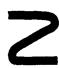
\includegraphics[keepaspectratio]{images/part002_5aba953c.jpg}}

In general, the dual of \(L^{\infty}\) is not isomorphic to \(L^{1}\) , consequently \(L^{1}\) and \(L^{\infty}\) are not reflexive (Exer. 10). We are going to characterize the continuous linear forms on \(L^{\infty}\) that arise, by passage to the quotient, from a linear form \(g \mapsto \int fg d\mu\) on \(L^{\infty}\) , where \(g \in L^{1}\) .

The ordered vector space \(\mathrm{L}^{\infty}(\mathrm{T},\mu)\) , which is a subspace of \(\mathrm{L}_{\mathrm{loc}}^{1}(\mathrm{T},\mu)\) , is fully lattice-ordered; for, if \((f_{\alpha})\) is a family of positive functions in \(L^{\infty}\) whose set of classes \((\dot{f}_{\alpha})\) is bounded above in \(L^{\infty}\) , there exists an \(a\geqslant0\) such that \(\mathrm{N}_{\infty}(f_{\alpha})\leqslant a\) for all \(\alpha\) . Since \(\mathrm{L}_{\mathrm{loc}}^{1}(\mathrm{T},\mu)\) is fully lattice-ordered, the family \((\dot{f}_{\alpha})\) admits a supremum \(\dot{h}\) in \(\mathrm{L}_{\mathrm{loc}}^{1}(\mathrm{T},\mu)\) ; but since \(\dot{a}\geqslant\dot{f}_{\alpha}\) for every \(\alpha\) , we have \(\dot{h}\leqslant\dot{a}\) , consequently \(\mathrm{N}_{\infty}(h)\leqslant a\) , whence our assertion.

PROPOSITION 14. --- In order that a positive linear form \(\theta\) on \(\mathcal{L}^{\infty}\) be of the type \(f \mapsto \int fg d\mu\) , where \(g \in \mathcal{L}^{1}\) , it is necessary and sufficient that, for every increasing directed family \((f_{\alpha})_{\alpha \in \mathrm{A}}\) of positive functions in \(\mathcal{L}^{\infty}\) whose set of classes \((\dot{f}_{\alpha})_{\alpha \in \mathrm{A}}\) is bounded above in \(\mathrm{L}^{\infty}\) and admits \(\dot{h}\) as its supremum in this space, one have

\[
\theta (h) = \sup _ {\alpha \in \mathrm{A}} \theta (f _ {\alpha}).
\]

Let us first show that the condition is necessary. The measure \(h \cdot \mu\) is the supremum in \(\mathcal{M}(\mathrm{T})\) of the set of measures \(f_{\alpha} \cdot \mu\) (No.~5, Scholium); therefore (Ch. II, §2, No.~2), for every function \(\varphi \geqslant 0\) in \(\mathcal{K}(\mathrm{T})\) , we have \(\int h\varphi d\mu = \sup_{\alpha \in \mathrm{A}} \int f_{\alpha}\varphi d\mu\) . If now \(a\) is a number \(\geqslant 0\) such that \(\mathrm{N}_{\infty}(f_{\alpha}) \leqslant a\) for all \(\alpha \in \mathrm{A}\) (which implies that \(\mathrm{N}_{\infty}(h) \leqslant a\) ), then for every \(\varepsilon > 0\) there exists a \(\varphi \in \mathcal{K}(\mathrm{T})\) such that \(\varphi \geqslant 0\) and \(\mathrm{N}_1(g - \varphi) \leqslant \varepsilon\) , from which we infer that \(\int f_{\alpha}|g - \varphi| d\mu \leqslant a\varepsilon\) for all \(\alpha \in \mathrm{A}\) , and \(\int h|g - \varphi| d\mu \leqslant a\varepsilon\) . Since \(\sup_{\alpha \in \mathrm{A}} \int f_{\alpha}g d\mu \leqslant \int hg d\mu\) , this proves that the two members of this inequality are equal.

To establish that the condition is sufficient, we shall make use of the following lemma:

Lemma 4. --- \(1^{\circ}\) Let \(f\) be a lower semi-continuous and bounded positive function on \(\mathbf{T}\) . Then its class \(\dot{f}\) in \(\mathbf{L}^{\infty}\) is the supremum of the set of classes \(\dot{\varphi}\) , where \(\varphi\) runs over the set of functions in \(\mathcal{K}(\mathbf{T})\) such that \(0 \leqslant \varphi \leqslant f\) .

\(2^{\circ}\) Let \(f\) be a measurable and bounded positive function on \(\mathbf{T}\) . Then its class \(\dot{f}\) in \(\mathrm{L}^{\infty}\) is the infimum of the set of classes \(\dot{\psi}\) , where \(\psi\) runs over the set of lower semi-continuous and bounded functions on \(\mathbf{T}\) that are \(\geqslant f\) .

\(1^{\circ}\) Let \(f'\) be a function in \(\mathcal{L}^{\infty}\) such that \(\dot{f}'\) is the supremum in \(\mathrm{L}^{\infty}\) of the set of classes \(\dot{\varphi}\) of the functions \(\varphi\) in \(\mathcal{K}(\mathrm{T})\) such that \(0 \leqslant \varphi \leqslant f\) ; obviously \(\dot{f}' \leqslant \dot{f}\) . Let U be a relatively compact open subset of T; for every function \(h\) in \(\mathcal{K}(\mathrm{T})\) such that \(0 \leqslant h \leqslant f\varphi_{\mathrm{U}}\) one has, by definition, \(h(t) \leqslant f'(t)\) locally almost everywhere, therefore \(h(t) \leqslant f'(t)\varphi_{\mathrm{U}}(t)\) almost everywhere; it follows that \(\int h d\mu \leqslant \int f'\varphi_{\mathrm{U}} d\mu\) . However, since \(f\varphi_{\mathrm{U}}\) is lower semi-continuous, \(\int f\varphi_{\mathrm{U}} d\mu = \sup \int h d\mu\) , where \(h\) runs over the set of functions in \(\mathcal{K}(\mathrm{T})\) such that \(0 \leqslant h \leqslant f\varphi_{\mathrm{U}}\) (Ch. IV, §1, No.~1, Def. 1); therefore

\[
\int f \varphi_ {\mathrm{U}} d \mu \leqslant \int f ^ {\prime} \varphi_ {\mathrm{U}} d \mu ,
\]

and since \(f' \varphi_{\mathrm{U}} \leqslant f \varphi_{\mathrm{U}}\) almost everywhere, necessarily \(f \varphi_{\mathrm{U}} = f' \varphi_{\mathrm{U}}\) almost everywhere, whence \(f = f'\) locally almost everywhere.

\(2^{\circ}\) Let \(f'\) be a function in \(\mathcal{L}^{\infty}\) such that \(\dot{f}'\) is the infimum in \(\mathrm{L}^{\infty}\) of the set of classes \(\dot{\psi}\) of the lower semi-continuous functions \(\psi\) that are bounded and \(\geqslant f\) ; then \(\dot{f}' \geqslant \dot{f}\) . Let K be a compact subset of T; for every lower semi-continuous function h that is bounded and \(\geqslant f\varphi_{K}\) , let \(\overline{h}\) be the function equal to h on K and to \(\|f\| + \|h\|\) on T - K. Then \(\overline{h}\) is lower semi-continuous and \(\geqslant f\) , therefore by definition \(\overline{h}(t) \geqslant f'(t)\) locally almost everywhere; it follows that \(h(t) \geqslant f'(t)\varphi_{\mathrm{K}}(t)\) almost everywhere, whence \(\int h d\mu \geqslant \int f'\varphi_{K} d\mu\) . But \(\int f\varphi_{K} d\mu = \inf \int h d\mu\) , where h runs over the set of lower semi-continuous functions that are bounded and \(\geqslant f\varphi_{K}\) (Ch. IV, §1, No.~3, Def. 3); therefore

\[
\int f \varphi_ {\mathrm{K}} d \mu \geqslant \int f ^ {\prime} \varphi_ {\mathrm{K}} d \mu ,
\]

and since \(f\varphi_{\mathrm{K}} \leqslant f'\varphi_{\mathrm{K}}\) almost everywhere, necessarily \(f\varphi_{\mathrm{K}} = f'\varphi_{\mathrm{K}}\) almost everywhere, whence \(f = f'\) locally almost everywhere.

The lemma having been proved, let \(\theta\) be a positive linear form on \(\mathcal{L}^{\infty}\) satisfying the condition in the statement of Prop. 14. The restriction of \(\theta\) to the space \(\mathcal{K}(\mathrm{T})\) is a positive measure \(\nu\) on \(\mathrm{T}\) . We are going to show that, for every positive function \(f\in \mathcal{L}^{\infty}(\mathrm{T},\mu)\) , one has \(\theta (f) = \nu^{*}(f)\) . Suppose first that \(f\) is lower semi-continuous (and bounded); by Lemma 4, \(\dot{f}\) is the supremum of the increasing directed set of classes \(\dot{\varphi}\) , where \(\varphi\) runs over the directed set \(\Phi\) of functions in \(\mathcal{K}(\mathrm{T})\) such that \(0\leqslant \varphi \leqslant f\) . Since by hypothesis \(\theta (f) = \sup_{\varphi \in \Phi}\theta (\varphi)\) , and \(\nu^{*}(f) = \sup_{\varphi \in \Phi}\nu (\varphi)\) by definition, our assertion is proved in this case. Secondly, suppose that \(f\) is \(\mu\) -measurable and bounded; then, by definition, \(\nu^{*}(f) = \inf_{\psi \in \Psi}\nu^{*}(\psi)\) , where \(\psi\) runs over the decreasing directed set \(\Psi\) of lower semi-continuous functions that are bounded and \(\geqslant f\) . If \(a\geqslant \| f\|\) then, applying the hypothesis of the statement to the increasing directed set of classes of the functions \(a - \psi\) , where \(\psi \in \Psi\) and \(\psi \leqslant a\) , one sees, by virtue of the lemma, that \(\theta (f) = \inf_{\psi \in \Psi}\theta (\psi)\) , therefore indeed \(\theta (f) = \nu^{*}(f)\) . In particular, for every \(\mu\) -negligible function \(f\geqslant 0\) , one has \(\theta (f) = 0\) , therefore \(\nu^{*}(f) = 0\) and consequently (No.~5, Th. 2) \(\nu\) is a measure with base \(\mu\) ; moreover, \(\nu^{*}(1) = \theta (1) < +\infty\) , consequently (Cor. of Th. 1) \(\nu = g\cdot \mu\) with \(g\in \mathcal{L}^1 (\mathrm{T},\mu)\) . Finally, since every \(\mu\) -measurable function is \(\nu\) -measurable, every positive function \(f\in \mathcal{L}^{\infty}(\mathrm{T},\mu)\) is \(\nu\) -integrable and \(\int fg d\mu = \nu^{*}(f) = \theta (f)\) , which completes the proof.

One concludes from Prop. 14 that the linear forms on \(\mathcal{L}^{\infty}\) of the type \(f\mapsto \int fg d\mu\) , where \(g\in \mathcal{L}^{1}\) , are the differences \(\theta_{1} - \theta_{2}\) , where \(\theta_{1}\) and \(\theta_{2}\) are positive linear forms satisfying the condition of Prop. 14.

\subsection{Applications: II. Functions of measures}

Let \(\mu_1, \mu_2, \ldots, \mu_n\) be real measures on \(T\) , and let \(u(x_1, \ldots, x_n)\) be a finite numerical function, defined on \(\mathbf{R}^n\) , and positively homogeneous, that is (Ch. I, §1, No.~1), such that

\[
u (\alpha x _ {1}, \ldots , \alpha x _ {n}) = \alpha u (x _ {1}, \ldots , x _ {n})\tag{12}
\]

for every scalar \(\alpha \geqslant 0\) . There exist positive measures \(\lambda\) on T such that \(|\mu_i| \leqslant \lambda\) for \(1 \leqslant i \leqslant n\) (for example, the sum \(\sum_{i=1}^{n} |\mu_i|\) ). Let \(\lambda\) and \(\lambda'\) be two such measures on T. One can write \(\mu_i = f_i \cdot \lambda = f_i' \cdot \lambda'\) , where \(f_i\) (resp. \(f_i'\) ) is measurable and essentially bounded for the measure \(\lambda\) (resp. \(\lambda'\) ) (No.~5, Th. 2). We are going to establish the following result: in order that the numerical function \(u(f_1, \ldots, f_n)\) be locally integrable for \(\lambda\) , it is necessary and sufficient that the function \(u(f_1', \ldots, f_n')\) be locally integrable for \(\lambda'\) , in which case

\[
u (f _ {1}, \dots , f _ {n}) \cdot \lambda = u (f _ {1} ^ {\prime}, \dots , f _ {n} ^ {\prime}) \cdot \lambda^ {\prime}.
\]

Since \(|\mu_i| \leqslant \inf(\lambda, \lambda')\) , we can restrict ourselves to the case that \(\lambda \leqslant \lambda'\) . Then \(\lambda = g \cdot \lambda'\) , where \(g\) is a \(\lambda'\) -measurable function such that \(0 \leqslant g \leqslant 1\) (No.~5, Th. 2); whence (No.~4, Prop. 8)

\[
\mu_ {i} = f _ {i} \cdot (g \cdot \lambda^ {\prime}) = (f _ {i} g) \cdot \lambda^ {\prime};
\]

it follows (No.~3, Cor. 2 of Prop. 3) that \(f_{i}g\) is equal to \(f_{i}'\) locally almost everywhere for \(\lambda'\) . Consequently, by (12),

\[
u (f _ {1} ^ {\prime}, \dots , f _ {n} ^ {\prime}) = u (f _ {1} g, \dots , f _ {n} g) = u (f _ {1}, \dots , f _ {n}) g
\]

locally almost everywhere for \(\lambda'\) . In order that \(u(f_1', \ldots, f_n')\) be locally \(\lambda'\) -integrable, it is therefore necessary and sufficient that \(u(f_1, \ldots, f_n)g\) be locally integrable for \(\lambda'\) , therefore (No.~4, Prop. 8) that \(u(f_1, \ldots, f_n)\) be locally integrable for \(\lambda\) ; and then (No.~4, Prop. 8)

\[
u \left(f _ {1} ^ {\prime}, \dots , f _ {n} ^ {\prime}\right) \cdot \lambda^ {\prime} = \left(u \left(f _ {1}, \dots , f _ {n}\right) g\right) \cdot \lambda^ {\prime} = u \left(f _ {1}, \dots , f _ {n}\right) \cdot \lambda .
\]

Thus, the measure \(u(f_{1},\ldots,f_{n})\cdot\lambda\) depends only on the measures \(\mu_{1},\ldots,\mu_{n}\) and the function u; it is also denoted \(u(\mu_{1},\ldots,\mu_{n})\) . This measure is therefore defined whenever u is a positively homogeneous function such that, for a positive measure \(\lambda\) that is an upper bound for all of the \(|\mu_{i}|\) , \(u(f_{1},\ldots,f_{n})\) is locally \(\lambda\) -integrable, where \(f_{i}\) denotes the density of \(\mu_{i}\) with respect to \(\lambda\) . Note that this condition is fulfilled when u is positively homogeneous and continuous: for, one then has

\[
\left| u \left(x _ {1}, \dots , x _ {n}\right) \right| \leqslant a \left(\left| x _ {1} \right| + \left| x _ {2} \right| + \dots + \left| x _ {n} \right|\right)
\]

(u being bounded in a sufficiently small neighborhood of \((0,\ldots,0)\) ), and since \(u(f_{1},\ldots,f_{n})\) is \(\lambda\) -measurable (Ch. IV, §5, No.~3, Th. 1), it is locally \(\lambda\) -integrable by virtue of the criterion for integrability (Ch. IV, §5, No.~6, Th. 5).

Let \(u_1, \ldots, u_p\) be positively homogeneous numerical functions defined on \(\mathbf{R}^n\) , such that the \(p\) functions \(g_k = u_k(f_1, \ldots, f_n)\) ( \(1 \leqslant k \leqslant p\) ) are locally \(\lambda\) -integrable. Let \(v\) be a positively homogeneous numerical function defined on \(\mathbf{R}^p\) such that \(v(g_1, \ldots, g_p)\) is locally \(\lambda\) -integrable. Set

\[
w (x _ {1}, \ldots , x _ {n}) = v \big (u _ {1} (x _ {1}, \ldots , x _ {n}), \ldots , u _ {p} (x _ {1}, \ldots , x _ {n}) \big).
\]

Then, the function w is positively homogeneous, \(w(f_{1}, \ldots, f_{n})\) is locally \(\lambda\) -integrable and, by definition,

\[
w \left(\mu_ {1}, \dots , \mu_ {n}\right) = v \left(u _ {1} \left(\mu_ {1}, \dots , \mu_ {n}\right), \dots , u _ {p} \left(\mu_ {1}, \dots , \mu_ {n}\right)\right).
\]

In the special case of the functions \(x^{+}\) , \(x^{-}\) , \(|x|\) , \(x + y\) , \(\inf(x, y)\) , \(\sup(x, y)\) , the measures defined by the procedure just described coincide, respectively, with those that have been denoted \(\mu^{+}\) , \(\mu^{-}\) , \(|\mu|\) , \(\mu + \nu\) , \(\inf(\mu, \nu)\) , \(\sup(\mu, \nu)\) ; this follows at once from the Cor. of Prop. 2 of No.~2. If \(\mu\) and \(\nu\) are two real measures, and \(\theta = \mu + i\nu\) , then \(|\theta| = \sqrt{\mu^{2} + \nu^{2}}\) ; for, let \(\lambda\) be a measure \(\geqslant 0\) that is an upper bound for \(|\mu|\) and \(|\nu|\) , and let f, g be locally \(\lambda\) -integrable functions such that \(\mu = f \cdot \lambda\) , \(\nu = g \cdot \lambda\) ; then

\[
\sqrt {\mu^ {2} + \nu^ {2}} = \sqrt {f ^ {2} + g ^ {2}} \cdot \lambda ,
\]

\(\theta = (f + ig) \cdot \lambda\) , therefore (No.~2, Prop. 2) \(|\theta| = \sqrt{f^2 + g^2} \cdot \lambda\) .

This method can be applied to the positively homogeneous function \((x_1^2 +\ldots +x_n^2)^{1 / 2}\) to define the length of a curve in \(\mathbf{R}^n\)

\subsection{Diffuse measures; atomic measures}

DEFINITION 5. --- A measure \(\theta\) on T is said to be diffuse if \(|\theta|(\{t\}) = 0\) for every \(t \in \mathrm{T}\) .

Example. --- Lebesgue measure on \(\mathbf{R}\) is diffuse (Ch. IV, §1, No.~3, Remark 1).

To say that \(\theta\) is a diffuse measure on T amounts to saying that every set with finite complement carries \(|\theta|\) , or again that \(|\theta|\) is alien to every point measure. The diffuse measures therefore form a band in \(\mathcal{M}(\mathrm{T})\) (Ch. II, §1, No.~5, Th. 1).

Recall (Ch. III, §1, No.~3) that a complex measure \(\rho\) on T is said to be atomic if it is of the form \(\sum_{t\in \mathrm{T}}\alpha (t)\varepsilon_t\) , where \(\alpha\) is a complex function on T such that \(\sum_{t\in \mathrm{K}}|\alpha (t)| < +\infty\) for every compact subset K of T, which expresses that the family \(\left(\alpha (t)\varepsilon_t\right)_{t\in \mathrm{T}}\) is summable (§2, No.~1, Remark 2). It then follows from the remark following Cor. 3 of Th. 2 of No.~5 that \(|\rho| = \sum_{t\in \mathrm{T}}|\alpha (t)|\varepsilon_t\) . The function \(\alpha\) that occurs in these formulas is uniquely determined, because \(\alpha (t) = \rho (\{t\})\) . An atomic measure and a diffuse measure are alien to each other.

PROPOSITION 15. --- Every complex measure \(\sigma\) on T may be written in one and only one way in the form \(\rho + \theta\) , where \(\rho\) is an atomic measure and \(\theta\) is a diffuse measure; one then has \(|\sigma| = |\rho| + |\theta|\) .

The uniqueness of the decomposition is obvious since, \(\rho\) being atomic and \(\theta\) diffuse, necessarily \(\rho = \sum_{t\in \mathrm{T}}\rho (\{t\})\varepsilon_t = \sum_{t\in \mathrm{T}}\sigma (\{t\})\varepsilon_t\) and \(\theta = \sigma -\rho\) . To establish existence, it suffices to observe that \(\sum_{t\in \mathrm{K}}|\sigma (\{t\})| \leqslant |\sigma |(\mathrm{K}) < +\infty\) for every compact set \(\mathbf{K}\) , so that one can set \(\sum_{t\in \mathrm{T}}\sigma (\{t\})\varepsilon_t = \rho\) . The measure \(\sigma -\rho\) is obviously diffuse, and the relation \(|\sigma | = |\rho | + |\sigma -\rho |\) follows at once from Cor. 3 of Prop. 13 of No.~7.

One observes that this proof shows that if \(\sigma\) is carried by a set \(M\) and if \(|\sigma| (\{t\}) > 0\) for every \(t \in M\) , then \(\sigma\) is atomic.

\section{IMAGES OF A MEASURE}

\subsection{Image of a positive measure}

Let X be a locally compact space, \(\pi\) a \(\mu\) -measurable mapping of T into X. To say that the pair \((\pi,1)\) is \(\mu\) -adapted (§4, No.~1) is equivalent to saying that for every function \(f \in \mathcal{K}(X)\) , the function \(f \circ \pi\) is essentially \(\mu\) -integrable.

PROPOSITION 1. --- Let \(\pi\) be a \(\mu\) -measurable mapping of T into a locally compact space X. The following two properties are equivalent:

\begin{enumerate}
\def\labelenumi{\alph{enumi})}
\item
  for every function \(f \in \mathcal{K}(\mathrm{X})\) , \(f \circ \pi\) is essentially \(\mu\) -integrable.
\item
  for every compact set \(\mathrm{K}\subset \mathrm{X}\) , \(\overline{\pi} (\mathrm{K})\) is essentially \(\mu\) -integrable.
\end{enumerate}

We have just observed that a) implies that the pair \((\pi,1)\) is \(\mu\) -adapted. Consequently ( \(\S4\) , No.~4, Th. 2), for every compact set \(K\subset X\) , the function \(\varphi_{K}\circ\pi=\varphi_{A}\) , where \(A=\overline{\pi}(K)\) , is essentially \(\mu\) -integrable, in other words, a) implies b).

Conversely, suppose that \(\overline{\pi}^{1}(K)\) is essentially \(\mu\) -integrable for every compact subset K of X, and let us show that a) is verified. Indeed, let S be the support of f; since S is compact, setting \(A = \overline{\pi}^{1}(S)\) we have, by hypothesis,

\[
\int^ {\bullet} \left| f (\pi (t)) \right| d \mu (t) \leqslant \| f \| \int^ {\bullet} \varphi_ {\mathrm{S}} (\pi (t)) d \mu (t) = \| f \| \int^ {\bullet} \varphi_ {\mathrm{A}} (t) d \mu (t) <   + \infty .
\]

Since \(f \circ \pi\) is \(\mu\) -measurable (Ch. IV, §5, No.~3, Th. 1), we see that \(f \circ \pi\) is essentially \(\mu\) -integrable (§1, No.~3, Prop. 9).

Property b) is obviously equivalent to the following (which is therefore also equivalent to a)):

\begin{enumerate}
\def\labelenumi{\alph{enumi})}
\setcounter{enumi}{2}
\tightlist
\item
  For every point \(x\) of \(X\) , there exists a neighborhood \(V\) of \(x\) such that \(\overline{\pi}^1(V)\) is essentially \(\mu\) -integrable.
\end{enumerate}

DEFINITION 1. --- Let \(\mu\) be a positive measure on a locally compact space T. A mapping \(\pi\) of T into a locally compact space X is said to be \(\mu\) -proper (or proper for the measure \(\mu\) ) if the pair \((\pi,1)\) is \(\mu\) -adapted, that is (§4, No.~1), if \(\pi\) is \(\mu\) -measurable and satisfies the (equivalent) conditions of Prop. 1. The measure \(\int \varepsilon_{\pi(t)} d\mu(t)\) on X is then called the image of \(\mu\) under \(\pi\) and is denoted \(\pi(\mu)\) .

Thus if \(\nu = \pi (\mu)\) then, by definition, for \(f\in \mathcal{K}(\mathbf{X})\) one has

\[
\int f (x) d \nu (x) = \int f (\pi (t)) d \mu (t).\tag{1}
\]

Remarks. --- 1) If \(\mu\) is bounded (in particular, if \(\mu\) has compact support) then every \(\mu\) -measurable mapping of T into X is \(\mu\) -proper (Ch. IV, §5, No.~3, Th. 1 and No.~6, Th. 5).

\begin{enumerate}
\def\labelenumi{\arabic{enumi})}
\setcounter{enumi}{1}
\item
  If \(\pi\) is \(\mu\) -measurable and if, for every compact subset \(K\) of \(X\) , \(\overline{\pi}^{1}(K)\) is relatively compact, then \(\pi\) is \(\mu\) -proper (Ch. IV, §5, No.~5, Prop. 7 and No.~6, Th. 5); in particular, every proper continuous mapping of \(T\) into \(X\) (GT, I, §10, No.~2, Th. 1) is \(\mu\) -proper for every positive measure \(\mu\) on \(T\) . More particularly, this is true of every homeomorphism \(\pi\) of \(T\) onto X; the measure \(\nu = \pi(\mu)\) is then none other than the measure on X that is the transport of \(\mu\) by \(\pi\) (Ch. III, §1, No.~3).
\item
  Suppose that the topology of X admits a countable base; then every mapping \(\pi\) of T into X that satisfies condition b) of Prop. 1 is \(\mu\) -measurable, hence is \(\mu\) -proper. It suffices to apply Th. 4 of Ch. IV, §5, No.~5, on observing that X is then metrizable (GT, IX, §2, No.~9, Cor. of Prop. 16) and that, for any metric compatible with the topology of X, every closed ball is a countable union of compact sets.
\end{enumerate}

\subsection{Integration with respect to the image of a positive measure}

Let \(\pi\) be a \(\mu\) -proper mapping of T into X, and let \(\nu = \pi(\mu)\) . Applying the results of §4, one obtains the following statements:

PROPOSITION 2. --- For every numerical function \(f \geqslant 0\) defined on X,

\[
\int^ {\bullet} f (x) d \nu (x) = \int^ {\bullet} f (\pi (t)) d \mu (t).\tag{2}
\]

This follows from Th. 1 of §4, No.~2.

COROLLARY 1. --- For every subset A of X,

\[
\nu^ {\bullet} (\mathrm{A}) = \mu^ {\bullet} \left(\overline {{\pi}} ^ {- 1} (\mathrm{A})\right).
\]

COROLLARY 2. --- For a subset A of X to be locally negligible for \(\nu\) , it is necessary and sufficient that \(\overline{\pi}^{-1}(\mathrm{A})\) be locally negligible for \(\mu\) .

COROLLARY 3. --- If the measure \(\mu\) is concentrated on a set M, then \(\pi(\mu)\) is concentrated on \(\pi(M)\) .

For, if \(\mathrm{N} = \mathrm{X} - \pi(\mathrm{M})\) then \(\overline{\pi}^1(\mathrm{N})\) does not intersect \(\mathrm{M}\) , therefore is locally \(\mu\) -negligible, consequently (Cor. 2) \(\mathrm{N}\) is locally \(\nu\) -negligible.

COROLLARY 4. --- Let S be the support of \(\mu\) . If \(\pi\) is continuous, then the support of \(\pi(\mu)\) is \(\overline{\pi(S)}\) .

For, it follows from Cor. 3 that \(\pi(\mu)\) is concentrated on \(\pi(S)\) , therefore if \(S'\) is the support of \(\pi(\mu)\) then \(S' \subset \overline{\pi(S)}\) . On the other hand, \(\overline{\pi}(X - S')\) is a locally \(\mu\) -negligible open set (Cor. 2), hence is \(\mu\) -negligible (Ch. IV, §5, No.~2, Cor. 2 of Prop. 5). Therefore \(\overline{\pi}(X - S') \subset T - S\) , consequently \(\pi(S) \subset S'\) , which proves the corollary.

PROPOSITION 3. --- For a mapping f of X into a topological space G to be ν-measurable, it is necessary and sufficient that \(f \circ \pi\) be μ-measurable.

This is an immediate consequence of Prop. 3 of §4, No.~3.

COROLLARY. --- For a subset A of X to be \(\nu\) -measurable, is is necessary and sufficient that \(\overline{\pi}^{1}(A)\) be \(\mu\) -measurable.

\pandocbounded{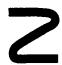
\includegraphics[keepaspectratio]{images/part002_e5542695.jpg}}

However, the image under \(\pi\) of a \(\mu\) -measurable subset M of T is not necessarily \(\nu\) -measurable, even if \(\pi\) is continuous and M is \(\mu\) -negligible (Exer. 7 and §8, Exer. 1).

THEOREM 1. --- Let f be a function defined on X with values in \(\overline{R}\) or in a Banach space F. For f to be essentially \(\nu\) -integrable, it is necessary and sufficient that \(f \circ \pi\) be essentially \(\mu\) -integrable, in which case

\[
\int \mathbf {f} (x) d \nu (x) = \int \mathbf {f} (\pi (t)) d \mu (t).\tag{3}
\]

Suppose, moreover, that \(\pi\) is continuous and proper. Then, for \(\mathbf{f}\) to be \(\nu\) -integrable, it is necessary and sufficient that \(\mathbf{f} \circ \pi\) be \(\mu\) -integrable.

It suffices to apply Th. 2 of §4, No.~4.

COROLLARY. --- For a subset A of X to be essentially \(\nu\) -integrable, it is necessary and sufficient that \(\overline{\pi}^{1}(A)\) be essentially \(\mu\) -integrable, in which case \(\nu(A)=\mu\left(\overline{\pi}^{1}(A)\right)\) .

In particular, for every compact set \(K \subset X\) , \(\nu(K) = \mu\left(\overline{\pi}(K)\right)\) . It follows from this and Cor. 3 of Prop. 2 that if \(\mu\) is atomic ( \(\S5\) , No.~10) then so is \(\pi(\mu) = \nu\) . For, let M be the set of \(t \in T\) such that \(\mu(\{t\}) \neq 0\) ; since \(\mu\) is carried by M, \(\nu\) is carried by \(\pi(M)\) ; moreover, for every \(x \in \pi(M)\) we have \(\nu(\{x\}) = \mu\left(\overline{\pi}(x)\right) > 0\) , since \(\overline{\pi}(x)\) contains at least one point of M. Therefore \(\nu\) is atomic ( \(\S5\) , No.~10, Prop. 15).

\subsection{Properties of the image of a positive measure}

PROPOSITION 4. --- Let T, T', T'' be three locally compact spaces, μ a positive measure on T, π a μ-measurable mapping of T into T', π' a mapping of T' into T'', and π'' = π' ∘ π.

\begin{enumerate}
\def\labelenumi{\alph{enumi})}
\item
  Suppose that \(\pi\) is \(\mu\) -proper and let \(\mu' = \pi(\mu)\) . For \(\pi'\) to be \(\mu'\) -proper, it is necessary and sufficient that \(\pi''\) be \(\mu\) -proper, in which case \(\pi''(\mu) = \pi'(\pi(\mu))\) (`transitivity of the image of a measure').
\item
  Suppose that \(\pi'\) is continuous, and that \(\pi''\) is \(\mu\) -proper; then \(\pi\) is \(\mu\) -proper, \(\pi'\) is \(\pi(\mu)\) -proper and \(\pi''(\mu) = \pi'(\pi(\mu))\) .
\end{enumerate}

Under the hypotheses of a), for \(\pi''\) to be \(\mu\) -measurable it is necessary and sufficient that \(\pi'\) be \(\mu'\) -measurable (No.~2, Prop. 3). On the other hand if K is a compact subset of \(T''\) , then \(\pi''(K) = \pi^{-1}(\pi'(K))\) ; for \(\pi''(K)\) to be essentially \(\mu\) -integrable, it is necessary and sufficient that \(\pi'(K)\) be essentially \(\mu'\) -integrable, by the Cor. of Th. 1. Finally, if \(\pi''\) is \(\mu\) -proper then, setting \(\mu'' = \pi''(\mu)\) , we have, for every function \(f \in \mathcal{K}(T'')\) ,

\[
\begin{array}{r l} \int f (t ^ {\prime \prime}) d \mu^ {\prime \prime} (t ^ {\prime \prime}) & = \int f (\pi^ {\prime \prime} (t)) d \mu (t) \\ & = \int f (\pi^ {\prime} (\pi (t))) d \mu (t) = \int f (\pi^ {\prime} (t ^ {\prime})) d \mu^ {\prime} (t ^ {\prime}) \end{array}
\]

by Th. 1 of No.~2, which completes the proof of a).

Under the hypotheses of b), let \(K'\) be a compact subset of \(T'\) . Then \(K'' = \pi'(K')\) is compact, therefore \(\overline{\pi''}(K'')\) is essentially \(\mu\) -integrable, therefore \(\overline{\pi}^{1}(K') \subset \overline{\pi''}(K'')\) is essentially \(\mu\) -integrable (Ch. IV, §5, No.~5, Prop. 7), so that \(\pi\) is \(\mu\) -proper. The proof is then concluded by applying part a) of the statement.

COROLLARY. --- Let T and T' be two locally compact spaces, \(\mu\) a positive measure on T, \(\pi\) a bijective mapping of T onto T', and \(\pi^{-1}\) the inverse mapping. Suppose that \(\pi\) is \(\mu\) -proper, and let \(\mu' = \pi(\mu)\) . Then \(\pi^{-1}\) is \(\mu'\) -proper and \(\pi^{-1}(\pi(\mu)) = \mu\) .

PROPOSITION 5. --- Let T and X be two locally compact spaces, \(\mu\) a positive measure on T, \(\pi\) a \(\mu\) -proper mapping of T into X, g a finite numerical function \(\geqslant 0\) , defined on X and such that \(g \circ \pi\) is locally integrable for \(\mu\) . In order that g be locally integrable for \(\pi(\mu)\) , it is necessary and sufficient that \(\pi\) be proper for the measure \((g \circ \pi) \cdot \mu\) , in which case

\[
\pi \big ((g \circ \pi) \cdot \mu \big) = g \cdot \pi (\mu).\tag{4}
\]

Set \(\nu = \pi(\mu)\) . For \(g\) to be locally \(\nu\) -integrable, it is necessary and sufficient that \(gf\) be \(\nu\) -integrable for every function \(f \in \mathcal{K}(X)\) ; since \(gf\) has compact support, it comes to the same to say that \(gf\) is essentially \(\nu\) -integrable, and this is equivalent to saying that \((g \circ \pi)(f \circ \pi)\) is essentially \(\mu\) -integrable (Th. 1). But, by Th. 1 of §5, No.~3, this signifies that \(f \circ \pi\) is essentially integrable for \(\rho = (g \circ \pi) \cdot \mu\) , and, by definition, this says that \(\pi\) is \(\rho\) -proper (since \(\pi\) is obviously \(\rho\) -measurable). Moreover,

\[
\int f g d \nu = \int f (\pi (t)) g (\pi (t)) d \mu (t) = \int f (\pi (t)) d \rho (t)
\]

(No.~2, Th. 1 and §5, Th. 1), which proves the relation (4).

PROPOSITION 6. --- Let T and X be two locally compact spaces, \((\lambda_{\alpha})_{\alpha\in\mathbb{A}}\) a family of positive measures on T, directed for the relation \(\leqslant\) , admitting in \(\mathcal{M}(\mathrm{T})\) a supremum \(\mu\) . In order that a mapping \(\pi\) of T into X be \(\mu\) -proper, it is necessary and sufficient that it be \(\lambda_{\alpha}\) -proper for all \(\alpha\in A\) , and that the family \(\left(\pi(\lambda_{\alpha})\right)_{\alpha\in\mathbb{A}}\) be bounded above in \(\mathcal{M}(\mathrm{X})\) . In this case,

\[
\pi (\mu) = \sup _ {\alpha} \pi (\lambda_ {\alpha}).\tag{5}
\]

For \(\pi\) to be \(\mu\) -measurable, it is necessary and sufficient that \(\pi\) be \(\lambda_{\alpha}\) -measurable for all \(\alpha \in A\) (§1, No.~4, Cor. 2 of Prop. 11). Suppose that this condition is satisfied; to say that \(\pi\) is \(\mu\) -proper is then equivalent to saying that, for every function \(f \in \mathcal{K}_{+}(X)\) ,

\[
\mu^ {\bullet} (f \circ \pi) <   + \infty .
\]

Now,

\[
\int^ {\bullet} (f \circ \pi) d \mu = \sup _ {\alpha} \int^ {\bullet} (f \circ \pi) d \lambda_ {\alpha} = \sup _ {\alpha} \int^ {\bullet} f d (\pi (\lambda_ {\alpha}))
\]

(§1, No.~4, Prop. 11); the first member is thus finite for every \(f \in \mathcal{K}_{+}(X)\) if and only if the family \((\pi(\lambda_{\alpha}))\) admits a supremum \(\theta\) in \(\mathcal{M}(X)\) , in which case \(\int(f \circ \pi) d\mu = \int f d\theta\) , a relation equivalent to (5).

COROLLARY 1. --- Let \((\mu_{\alpha})_{\alpha \in A}\) be a summable family of positive measures on T, such that \(\mu = \sum_{\alpha \in A} \mu_{\alpha}\) ; for a mapping \(\pi\) of T into a locally compact space X to be \(\mu\) -proper, it is necessary and sufficient that it be \(\mu_{\alpha}\) -proper for every \(\alpha \in A\) , and that the family \((\pi(\mu_{\alpha}))_{\alpha \in A}\) be summable. In this case,

\[
\pi (\mu) = \sum_ {\alpha \in A} \pi (\mu_ {\alpha}).\tag{6}
\]

COROLLARY 2. --- Let T and X be two locally compact spaces, \((\lambda_{i})_{1\leqslant i\leqslant n}\) a finite sequence of positive measures on T, and let \(\mu=\sum_{i=1}^{n}\lambda_{i}\) . For a mapping \(\pi\) of T into X to be \(\mu\) -proper, it is necessary and sufficient that it be \(\lambda_{i}\) -proper for every index i, in which case

\[
\sum_ {i = 1} ^ {n} \pi (\lambda_ {i}) = \pi \left(\sum_ {i = 1} ^ {n} \lambda_ {i}\right).
\]

\subsection{Image of a complex measure}

Let \(\theta\) be a complex measure on T, and let \(\pi\) be a mapping of T into a locally compact space X; suppose that \(\pi\) is \(\theta\) -measurable, and that for each \(f \in \mathcal{K}(X; \mathbf{C})\) , \(f \circ \pi\) is essentially \(\theta\) -integrable. Since it is equivalent to say that a function is measurable (resp. essentially integrable) with respect to \(\theta\) or with respect to \(|\theta|\) , this means that \(\pi\) is \(|\theta|\) -proper. If \(f \in \mathcal{K}(X; \mathbf{C})\) ,

\[
\left| \int (f \circ \pi) d \theta \right| \leqslant \int (| f | \circ \pi) d | \theta |;\tag{7}
\]

it follows at once that the linear form \(f \mapsto \int(f \circ \pi) d\theta\) on \(\mathcal{K}(X; \mathbf{C})\) is a complex measure on X (Ch. III, §1, No.~3, Prop. 6), and one can make the following definition:

DEFINITION 2. --- Let \(\theta\) be a complex measure on a locally compact space T. A mapping \(\pi\) of T into a locally compact space X is said to be \(\theta\) -proper if it is \(|\theta|\) -proper. The measure \(f \mapsto \int(f \circ \pi) d\theta\) is then called the image of \(\theta\) under \(\pi\) and is denoted \(\pi(\theta)\) .

The relation (7) may then be put in the following form:

\[
| \pi (\theta) | \leqslant \pi (| \theta |).\tag{8}
\]

The measure \(\pi(\theta)\) may be zero without \(\theta\) being zero, as one sees immediately on taking for T a space reduced to two points a, b, for \(\theta\) the measure \(\varepsilon_{a} - \varepsilon_{b}\) , and for \(\pi\) a constant mapping.

Let \(\theta\) and \(\theta'\) be two complex measures on T; if \(\pi\) is \(\theta\) -proper and \(\theta'\) -proper, it follows from Cor. 2 of Prop. 6 that \(\pi\) is \((\theta + \theta')\) -proper since \(|\theta + \theta'| \leqslant |\theta| + |\theta'|\) , and obviously \(\pi(\theta + \theta') = \pi(\theta) + \pi(\theta')\) .

In particular, if \(\theta\) is a real measure and \(\pi\) is \(\theta\) -proper, then

\[
\pi (\theta) = \pi (\theta^ {+}) - \pi (\theta^ {-}).\tag{9}
\]

Several results established earlier extend at once to complex measures; we cite the most important among them.

PROPOSITION 7. --- Let \(\theta\) be a complex measure on T, \(\pi\) a \(\theta\) -proper mapping of T into a locally compact space X, \(\nu\) the image measure \(\pi(\theta)\) .

\begin{enumerate}
\def\labelenumi{\alph{enumi})}
\item
  Let A be a subset of X; if \(\overline{\pi}^{1}(A)\) is locally \(\theta\) -negligible, then A is locally \(\nu\) -negligible.
\item
  Let \(f\) be a mapping of \(X\) into a topological space; if \(f \circ \pi\) is \(\theta\) -measurable, then \(f\) is \(\nu\) -measurable.
\item
  Let \(\mathbf{f}\) be a function defined on \(X\) , with values in a Banach space \(F\) ; if \(\mathbf{f} \circ \pi\) is essentially \(\theta\) -integrable, then \(\mathbf{f}\) is essentially \(\nu\) -integrable and
\end{enumerate}

\[
\int \mathbf {f} (\pi (t)) d \theta (t) = \int \mathbf {f} (x) d \nu (x).\tag{10}
\]

Taking into account formula (8), these results may be deduced from Cor. 2 of Prop. 2, from Prop. 3, and from Th. 1 of No.~2.

\subsection{Application: change of variable in the Lebesgue integral}

Let I be an interval (bounded or not) of R, a its left end-point and b its right end-point in \(\overline{R}\) , and \(\mu\) the Lebesgue measure on I. For every \(\mu\) -integrable function f and every interval \(H \subset I\) , with left end-point \(\alpha\) and right end-point \(\beta\) , we write \(\int_{\alpha}^{\beta} \mathbf{f}(t) dt\) instead of \(\int_{H} \mathbf{f}(t) dt = \int_{H} \mathbf{f} d\mu\) , and we set \(\int_{\beta}^{\alpha} \mathbf{f}(t) dt = -\int_{\alpha}^{\beta} \mathbf{f}(t) dt\) ; the meaning thus given to these symbols coincides with that attributed to them in FRV, II, §§1 and 2, when f is a regulated function with compact support (Ch. IV, §4, No.~4, Example).

Let \(g\) be a numerical function defined on \(I\) and locally \(\mu\) -integrable, \(x_0\) a point of \(I\) ; for every \(x \in I\) , set

\[
G (x) = c + \int_ {x _ {0}} ^ {x} g (t) d t \quad (c \text {   a   constant }).\tag{11}
\]

The numerical function G is continuous on I; this follows at once from Lebesgue's theorem (Ch. IV, §4, No.~3, Cor. 1 of Th. 2), since the product of g and the characteristic function of the interval with end-points x and \(x + h\) tends to a negligible function as h tends to 0. Therefore G(I) is an interval of R. Throughout this No., we will regard G as a mapping of I onto the locally compact space G(I). We denote by \(\lambda\) the measure \(g \cdot \mu\) on I.

Suppose first that g is \(\mu\) -integrable. Then, the same reasoning as above shows that the limits \(\mathrm{G}(a+)\) and \(\mathrm{G}(b-)\) exist and are finite; moreover, the measure \(|\lambda|\) is bounded ( \(\S5\) , No.~3, Cor. of Th. 1), and the mapping G of I into \(\mathrm{G}(\mathrm{I})\) is \(\lambda\) -proper.

PROPOSITION 8. --- Suppose g is \(\mu\) -integrable. If J denotes the open interval in R with end-points \(\mathrm{G}(a+)\) and \(\mathrm{G}(b-)\) , the image under G of the measure \(g \cdot \mu\) is the measure \(\varphi_{J} \cdot \nu\) if \(\mathrm{G}(a+) \leqslant \mathrm{G}(b-)\) and the measure \(-\varphi_{J} \cdot \nu\) if \(\mathrm{G}(a+) \geqslant \mathrm{G}(b-)\) (where \(\nu\) denotes Lebesgue measure on \(\mathrm{G}(\mathrm{I})\) ).

It suffices to prove that, for every function \(f \in \mathcal{K}\big(\mathrm{G}(\mathrm{I})\big)\) ,

\[
\int_ {\mathrm{G} (a +)} ^ {\mathrm{G} (b -)} f (\xi) d \xi = \int_ {a} ^ {b} f (\mathrm{G} (t)) g (t) d t.\tag{12}
\]

Now, this formula has already been proved for \(g \in \mathcal{K}(\mathrm{I})\) (FRV, II, §2, No.~1, formula (1)). Let us pass to the general case; there exists a sequence \((g_n)\) of functions in \(\mathcal{K}(\mathrm{I})\) such that: \(1^\circ\) the sequence \((g_n(t))\) tends to \(g(t)\) almost everywhere in I; \(2^\circ\) there exists a \(\mu\) -integrable function \(h \geqslant 0\) such that \(|g_n| \leqslant h\) for all \(n\) (Ch. IV, §3, No.~4, Th. 3). It follows at once from Lebesgue's theorem that, setting \(G_n(x) = c + \int_{x_0}^x g_n(t) dt\) , the sequence \((G_n)\) converges uniformly to G on I, and that the numbers \(G_n(a+)\) and \(G_n(b-)\) tend respectively to \(G(a+)\) and \(G(b-)\) . Let \(f'\) be a function in \(\mathcal{K}(\mathbf{R})\) that extends \(f\) ; the foregoing proves that \(f'(G_n(t))\) tends to \(f'(G(t)) = f(G(t))\) for all \(t \in \mathrm{I}\) ; applying Lebesgue's theorem, one sees that the formula (12) results from the formula

\[
\int_ {\mathrm{G} _ {n} (a +)} ^ {\mathrm{G} _ {n} (b -)} f ^ {\prime} (\xi) d \xi = \int_ {a} ^ {b} f ^ {\prime} \bigl (\mathrm{G} _ {n} (t) \bigr) g _ {n} (t) d t
\]

by passage to the limit.

COROLLARY. --- If a function f defined on G(I), with values in \(\overline{R}\) or in a Banach space, is such that the function \(t \mapsto \mathbf{f}(G(t))g(t)\) is integrable on I for Lebesgue measure, then f is integrable on J for Lebesgue measure and

\[
\int_ {\mathrm{G} (a +)} ^ {\mathrm{G} (b -)} \mathbf {f} (\xi) d \xi = \int_ {a} ^ {b} \mathbf {f} (\mathrm{G} (t)) g (t) d t\tag{13}
\]

(formula for change of variable in the Lebesgue integral).

For, \(\mathbf{f}\big(\mathrm{G}(t)\big)\) is integrable for the measure \(|g|\cdot\mu\) , hence also for the measures \(g^{+}\cdot\mu\) and \(g^{-}\cdot\mu\) ; it follows from Th. 1 (No.~2) that f is integrable for the image measures \(\mathrm{G}(g^{+}\cdot\mu)\) and \(\mathrm{G}(g^{-}\cdot\mu)\) , hence also for the measure \(\varphi_{J}\cdot\nu\) , and that (13) holds, on taking into account Prop. 8 and formula (9).

It can happen that \(\mathbf{f}\) is integrable on J for Lebesgue measure, but that \(t \mapsto \mathbf{f}(\mathbf{G}(t))g(t)\) is not integrable on I for Lebesgue measure (Exer. 10).

Now suppose that g maintains a constant sign almost everywhere (and is locally \(\mu\) -integrable); one may suppose for example that \(g(t) \geqslant 0\) almost everywhere in I. Then G is an increasing continuous function on I, therefore \(\mathrm{G}(a+)\) and \(\mathrm{G}(b-)\) exist (but may be infinite). Moreover, G is a \(\lambda\) -proper mapping of I into \(\mathrm{G}(\mathrm{I})\) : for, if \(\mathrm{G}(b-) \in \mathrm{G}(\mathrm{I})\) , there is an \(x_{1} \geqslant x_{0}\) such that G is constant for \(x \geqslant x_{1}\) , and then the inverse image under G of the compact interval \([G(x_{0}), G(b-)]\) is \(\lambda\) -integrable; if, on the contrary, \(G(b-) \notin G(I)\) , then the inverse image under G of every compact interval with left end-point \(G(x_{0})\) , contained in G(I), differs from a compact interval by at most a \(\lambda\) -negligible interval. One argues similarly for the compact intervals with right end-point \(G(x_{0})\) , whence our assertion. Moreover:

PROPOSITION 9. --- Suppose \(g \geqslant 0\) and locally \(\mu\) -integrable. Then, the image under \(G\) of the positive measure \(g \cdot \mu\) is Lebesgue measure on \(G(I)\) . For a function \(f\) , defined on \(G(I)\) , with values in \(\overline{R}\) or in a Banach space, to be integrable on \(G(I)\) for Lebesgue measure, it is necessary and sufficient that the function \(t \mapsto f(G(t))g(t)\) be integrable on \(I\) for Lebesgue measure, in which case the relation (13) holds.

The first part of the statement follows from the fact that the formula (12) is valid for every function \(f \in \mathcal{K}(\mathrm{G}(\mathrm{I}))\) ; for, the support of the function \(t \mapsto f(\mathrm{G}(t))\) is contained in an interval \(K \subset I\) on which g is integrable, by virtue of the above remarks, and it suffices to apply Prop. 8 to K. The second part is a consequence of Th. 1 of No.~2.

\subsection{Decomposition into slices. Inverse image of a measure under a local homeomorphism}

Let X be a locally compact space, \(\pi\) a mapping of X into a locally compact space T, \(\mu\) a positive measure on T, \(\Lambda: t \mapsto \lambda_t\) a scalarly essentially \(\mu\) -integrable and vaguely \(\mu\) -measurable mapping of T into \(\mathcal{M}_{+}(X)\) . Let \(\nu = \int \lambda_t d\mu(t)\) . If \(\lambda_t\) is carried by \(\overline{\pi}(t)\) for every \(t \in T\) , the equality \(\nu = \int \lambda_t d\mu(t)\) is said to be a decomposition into slices (or a disintegration) of \(\nu\) relative to \(\pi\) . This concept will be studied in detail in Ch. VI.

PROPOSITION 10. --- With the above notations, suppose that \(\pi\) is \(\nu\) -measurable. Let \(g\) be the function \(t \mapsto \lambda_t^*(1)\) on T. For \(\pi\) to be \(\nu\) -proper, it is necessary and sufficient that \(g\) be locally \(\mu\) -integrable, in which case

\[
\pi (\nu) = g \cdot \mu .\tag{14}
\]

We begin by arguing on the assumption that g is finite locally \(\mu\) -almost everywhere; we will rid ourselves of this auxiliary hypothesis at the end of the proof. Since \(\pi\) is by hypothesis \(\nu\) -measurable, to say that \(\pi\) is \(\nu\) -proper is equivalent to saying that \(\nu^{\bullet}(f\circ\pi)<+\infty\) for every function \(f\in\mathcal{K}_{+}(\mathrm{T})\) ; g being finite locally almost everywhere, we are under the conditions for applying assertion c) of Prop. 5 of §3, No.~2. Therefore

\[
\int^ {\bullet} (f \circ \pi) d \nu = \int^ {\bullet} d \mu (t) \int^ {\bullet} (f \circ \pi) d \lambda_ {t} = \int^ {\bullet} f (t) g (t) d \mu (t),
\]

from the fact that \(\lambda_{t}\) is concentrated on \(\overline{\pi}^{1}(t)\) . We know that g is \(\mu\) -measurable, since \(\Lambda\) is \(\mu\) -adequate ( \(\S3\) , No.~1, Def. 1). To say that the first member is finite for every \(f \in \mathcal{K}_{+}(\mathrm{T})\) is therefore equivalent to saying that g is locally \(\mu\) -integrable ( \(\S5\) , Prop. 1), and in this case (14) follows at once from the above relations.

It therefore only remains to eliminate the auxiliary hypothesis. If g is locally \(\mu\) -integrable, then g is finite locally \(\mu\) -almost everywhere, and the hypothesis is indeed satisfied. Let us assume that \(\pi\) is \(\nu\) -proper, and let us show that g is finite locally almost everywhere. Let \(\mathfrak{K}\) be the \(\mu\) -dense set of compact sets K such that \(\Lambda|K\) is vaguely continuous; since g is measurable, we are reduced to showing that every compact set \(K \in \mathfrak{K}\) such that \(g|K = +\infty\) is \(\mu\) -negligible. Now, let \(\mathcal{H}\) be the set of functions \(h \in \mathcal{K}_{+}(X)\) such that \(h \leqslant 1\) ; set \(g_{h}(t) = \lambda_{t}(h)\) , denote by \(\Lambda_{h}\) the \(\mu\) -adequate mapping \(t \mapsto h \cdot \lambda_{t}\) , by \(\nu_{h}\) the integral of \(\Lambda_{h}\) , and by f an element of \(\mathcal{K}_{+}(T)\) such that \(f \geqslant \varphi_{K}\) . Applying formula (14) to \(\Lambda_{h}\) , which does satisfy the auxiliary hypothesis, we obtain:

\[
\int (f \circ \pi) d \nu \geqslant \int (f \circ \pi) d \nu_ {h} = \int f g _ {h} d \mu .
\]

But the functions \(fg_h|K\) form an increasing directed set of continuous functions on \(K\) , whose upper envelope has the value \(+\infty\) ; by Dini's theorem (GT, X, §4, No.~1, Th. 1), one can choose \(h\) so that \(fg_h|K\) is greater than or equal to an arbitrary positive number \(n\) , and it follows that \(\int(f \circ \pi) d\nu \geqslant n \mu(K)\) . Since the first member is finite because \(\pi\) is \(\nu\) -proper, it then follows that \(\mu(K) = 0\) .

COROLLARY 1. --- Suppose that \(\pi\) is \(\nu\) -measurable.

\begin{enumerate}
\def\labelenumi{\alph{enumi})}
\item
  If \(\mathrm{N}\subset \mathrm{T}\) is locally \(\mu\) -negligible, then \(\overline{\pi}^{1}(\mathrm{N})\) is locally \(\nu\) -negligible.
\item
  If \(f\) is a \(\mu\) -measurable mapping of \(T\) into a topological space \(G\) , then \(f \circ \pi\) is \(\nu\) -measurable.
\end{enumerate}

We take up again the notations \(\Lambda_h\) , \(\nu_h\) , \(g_h\) of the end of the preceding proof: \(\nu_h\) being a bounded measure for every \(h \in \mathcal{H}\) , \(\pi\) is \(\nu_h\) -proper, \(g_h\) is locally \(\mu\) -integrable, and \(\pi(\nu_h) = g_h \cdot \mu\) , a measure with base \(\mu\) . It follows that N is locally negligible (resp. that \(f\) is measurable) for the measure \(\pi(\nu_h)\) ( \(\S 5\) , No.~3, Cor. 1 of Prop. 3 and Prop. 4). Consequently \(\overline{\pi}^1(N)\) is locally negligible (resp. \(f \circ \pi\) is measurable) for the measure \(\nu_h\) (Cor. 2 of

Prop. 2, resp. Prop. 3). Finally, one notes that the measures \(\nu_{h}\) form an increasing directed family of positive measures whose supremum is \(\nu\) , and one applies Cor. 1 (resp. Cor. 2) of Prop. 11 of §1, No.~4.

COROLLARY 2. --- Suppose that \(\pi\) is \(\nu\) -proper; let \(\mathbf{f}\) be a mapping defined on \(\mathbf{T}\) , with values in a Banach space or in \(\overline{\mathbf{R}}\) . For \(f \circ \pi\) to be essentially \(\nu\) -integrable, it is necessary and sufficient that \(gf\) be essentially \(\mu\) -integrable.

Taking into account Prop. 10, this follows immediately from Th. 1 of §5, No.~3 and Th. 1 of No.~2.

Example. --- Let X and T be two locally compact spaces, and let \(\pi\) be a local homeomorphism of X into T. In other words (GT, I, §11, Exer. 25), we assume that every point \(x \in X\) admits a neighborhood V such that \(\pi|V\) is a homeomorphism of V onto a neighborhood of \(\pi(x)\) ; if necessary replacing V by a relatively compact open neighborhood W of x such that \(\overline{W} \subset V\) , one deduces that the set \(\mathcal{U}\) of relatively compact open subsets U of X, such that \(\pi|\overline{U}\) is a homeomorphism of \(\overline{U}\) onto its image, is an open covering of X. Now let \(\mu\) be a positive measure on T; if U is an element of \(\mathcal{U}\), then \(\pi(U)\) is an open set in the compact space \(\pi(\overline{U})\) , therefore is a locally compact subspace of T, and one knows how to define the measure \(\mu|\pi(U)\) induced by \(\mu\) on \(\pi(U)\) (Ch. IV, §5, No.~7). Let \(\nu_{U}\) be the image of \(\mu|\pi(U)\) under the homeomorphism inverse to \(\pi|U\) ; we are going to show that there exists one and only one measure \(\nu\) on X that induces the measure \(\nu_{U}\) on every open set \(U \in \mathcal{U}\) . This measure is called the inverse image of \(\mu\) under the local homeomorphism \(\pi\) , and is denoted \(\overline{\pi}^{1}(\mu)\) .

The uniqueness of \(\nu\) follows at once from the principle of localization (Ch. III, §2, No.~1, Cor. of Prop. 1). To establish existence, we note that if \(t \in \mathbf{T}\) , then every point \(x \in \overline{\pi}^{-1}(t)\) admits a neighborhood that intersects \(\overline{\pi}^{-1}(t)\) only at the point \(x\) , so that \(\overline{\pi}^{-1}(t)\) is a discrete subspace of \(\mathbf{X}\) , and that the family \((\varepsilon_x)_{x \in \overline{\pi}^{-1}(t)}\) is summable; we denote its sum by \(\lambda_t\) . We next show that the mapping \(t \mapsto \lambda_t\) is scalarly essentially \(\mu\) -integrable, and that its integral \(\nu = \int \lambda_t d\mu(t)\) is the sought-for inverse image. This will result at once from the following lemma:

Lemma. --- a) Let \(f\) be an element of \(\mathcal{K}_{+}(X)\) ; the function \(t \mapsto \lambda_{t}(f)\) is positive, upper semi-continuous, with compact support, and its restriction to \(\pi(X)\) is continuous.

\begin{enumerate}
\def\labelenumi{\alph{enumi})}
\setcounter{enumi}{1}
\tightlist
\item
  Let U be an element of \(\mathcal{U}\), \(\nu\) the integral of the scalarly essentially \(\mu\) -integrable function \(t \mapsto \lambda_{t}\) ; the image of the measure \(\nu|U\) under \(\pi|U\) is equal to \(\mu|\pi(U)\) .
\end{enumerate}

To establish a), one may reduce by means of a partition of unity (Ch. III, §1, No.~2, Lemma 1) to the case that the support S of f is contained in an open set \(U \in \mathcal{U}\) . Let g be the mapping \(t \mapsto \lambda_{t}(f)\) ; \(\pi|U\) being a homeomorphism, \(g|\pi(U)\) belongs to \(\mathcal{K}_{+}(\pi(U))\) , consequently \((\pi(U)\) being an open set in \(\pi(X)\) ) the restriction of g to \(\pi(X)\) is continuous. Since g is positive and the restriction of g to the compact set \(\pi(S)\) is continuous, one sees that g is upper semi-continuous on T. It follows that g is \(\mu\) -integrable.

To establish b), denote by g an element of \(\mathcal{K}\big(\pi(\mathrm{U})\big)\) , by \(g^{\circ}\) its extension by 0 to T, by f the function \(g \circ (\pi|U)\) , and by \(f^{\circ}\) the extension by 0 of f to X. The assertion b) is equivalent to the equality \(\int g^{\circ} d\mu = \int f^{\circ} d\nu\) . But \(f \in \mathcal{K}(\mathrm{U})\) , therefore \(f^{\circ} \in \mathcal{K}(\mathrm{X})\) , and the second integral is therefore equal to \(\int \lambda_{t}(f^{\circ}) d\mu(t)\) . Finally \(\lambda_{t}(f^{\circ}) = g^{\circ}(t)\) , which completes the proof.

We now observe that \(\pi(\mathrm{X})\) is open in T, hence is \(\mu\) -measurable; the mapping \(\Lambda: t \mapsto \lambda_t\) is vaguely \(\mu\) -measurable, because its restriction to each of the sets \(\pi(\mathrm{X})\) and \(\mathbb{C}\pi(\mathrm{X})\) is vaguely continuous. Under these conditions, the formula \(\overline{\pi}^{1}(\mu) = \int \lambda_t d\mu(t)\) defines a decomposition into slices of \(\overline{\pi}^{1}(\mu)\) relative to \(\pi\) , and Prop. 10 yields the following result:

PROPOSITION 11. --- Let \(\pi\) be a local homeomorphism of a locally compact space \(X\) into a locally compact space \(T\) , and let \(\mu\) be a positive measure on \(T\) . Let \(n\) be the numerical function that associates to every \(t \in T\) the number of elements of \(\overline{\pi}^{1}(t)\) if this number is finite, and \(+\infty\) in the contrary case. For \(\pi\) to be \(\overline{\pi}^{1}(\mu)\) -proper, it is necessary and sufficient that \(n\) be locally \(\mu\) -integrable, in which case

\[
\pi \big (\bar {\pi} ^ {1} (\mu) \big) = n \cdot \mu .\tag{15}
\]

\section{INTEGRATION WITH RESPECT TO AN INDUCED MEASURE}

\subsection{Integration with respect to an induced measure}

Let X be a locally compact subspace of T, \(\mu\) a positive measure on T, and \(\mu_{X}\) the measure induced on X by \(\mu\) (Ch. IV, §5, No.~7). For every \(t \in T\) , let us define a measure \(\lambda_{t}\) on X in the following way: \(\lambda_{t} = \varepsilon_{t}\) if \(t \in X\) , \(\lambda_{t} = 0\) if \(t \in C X\) . For every finite numerical function g defined on X, \(\int g(x) d\lambda_{t}(x) = g(t)\) if \(t \in X\) and \(\int g(x) d\lambda_{t}(x) = 0\) if \(t \in C X\) . If g is a function in \(\mathcal{K}(X)\) we therefore have, by the definition of \(\mu_{X}\) ,

\[
\mu_ {\mathrm{X}} (g) = \int \langle g, \lambda_ {t} \rangle d \mu (t).\tag{1}
\]

This means that one can write

\[
\mu_ {\mathrm{X}} = \int \lambda_ {t} d \mu (t)\tag{2}
\]

(§3, No.~1).

Let us now define a mapping \(\pi\) of T into X by setting \(\pi(t) = t\) for \(t \in \mathbf{X}\) , and \(\pi(t) = t_0\) for \(t \in \mathbb{C} \mathbf{X}\) , \(t_0\) being an arbitrary point of \(\mathbf{X}\) ; one can write \(\lambda_t = \varphi_{\mathbf{X}}(t) \varepsilon_{\pi(t)}\) for every \(t \in \mathbf{T}\) . The mapping \(\pi\) is \(\mu\) -measurable, because its restrictions to \(\mathbf{X}\) and \(\mathbb{C} \mathbf{X}\) are (Ch. IV, §5, No.~10, Prop. 16); it follows at once that the pair \((\pi, \varphi_{\mathbf{X}})\) is \(\mu\) -adapted (§4, No.~1). We therefore have the following results:

PROPOSITION 1. --- For every numerical function \(g \geqslant 0\) defined on X,

\[
\int^ {\bullet} g d \mu_ {\mathrm{X}} = \int_ {\mathrm{X}} ^ {\bullet} g d \mu\tag{3}
\]

(cf.~§5, No.~3, Example, for the notation \(\int_{\mathbf{X}}^{\bullet}\) ).

Taking into account the preceding remarks and (2), the relation (3) follows from Th. 1 of §4.

COROLLARY 1. --- For every subset B of X, \(\mu_{\mathrm{X}}^{\bullet}(\mathrm{B}) = \mu^{\bullet}(\mathrm{B})\) ; for B to be locally \(\mu_{\mathrm{X}}\) -negligible, it is necessary and sufficient that B be locally \(\mu\) -negligible.

COROLLARY 2. --- Let M be a subset of T. If \(\mu\) is concentrated on M, then \(\mu_{X}\) is concentrated on \(M \cap X\) .

COROLLARY 3. --- For the measure \(\mu_{X}\) to be zero, it is necessary and sufficient that \(X\) be locally \(\mu\) -negligible.

Remark. --- If S is the support of \(\mu\) , then \(S \cap X\) (which is closed in X) contains the support of \(\mu_{X}\) by Cor. 2, but may be distinct from it. For example, if \(\mu\) is a diffuse measure and X is a subspace reduced to a point, then the induced measure \(\mu_{X}\) is zero, hence its support is empty. Note, however, that the support of \(\mu_{X}\) is equal to \(S \cap X\) if X is open in T.

PROPOSITION 2. --- For a mapping g of X into a topological space to be \(\mu_{X}\) -measurable, it is necessary and sufficient that g be \(\mu\) -measurable in X ( \(\S5\) , No.~3, Example).

This follows from Prop. 3 of §4.

COROLLARY. --- For a subset B of X to be \(\mu_{X}\) -measurable, it is necessary and sufficient that B be \(\mu\) -measurable.

THEOREM 1. --- Let g be a function defined on X, with values in \(\overline{R}\) or in a Banach space. For g to be essentially \(\mu_{X}\) -integrable, it is necessary and sufficient that \(\mathbf{g}\) be essentially \(\mu\) -integrable in X (§5, No.~3, Example), in which case

\[
\int \mathbf {g} d \mu_ {\mathrm{X}} = \int_ {\mathrm{X}} \mathbf {g} d \mu .\tag{4}
\]

This follows from Th. 2 of §4.

COROLLARY 1. --- For a subset B of X to be essentially \(\mu_{X}\) -integrable, it is necessary and sufficient that it be essentially \(\mu\) -integrable, in which case \(\mu_{\mathrm{X}}(\mathrm{B}) = \mu(\mathrm{B})\) .

COROLLARY 2. --- Let g be a complex function defined on T and locally \(\mu\) -integrable; the restriction \(g_{X}\) of g to X is then locally \(\mu_{X}\) -integrable, and

\[
(g \cdot \mu) _ {\mathrm{X}} = g _ {\mathrm{X}} \cdot \mu_ {\mathrm{X}}.\tag{5}
\]

This follows at once from Th. 1, applied to the functions \(fg_{\mathbf{X}}\) ( \(f \in \mathcal{K}(\mathbf{X}; \mathbf{C})\) ), and the definition of the measure induced on \(\mathbf{X}\) by a complex measure (Ch. IV, §5, No.~7).

COROLLARY 3. --- Let \(\theta\) be a complex measure on T; then

\[
| \theta | _ {\mathrm{X}} = | \theta_ {\mathrm{X}} |.\tag{6}
\]

Set \(|\theta| = \mu\) and apply Cor. 2 on taking \(g\) to be a complex function of absolute value 1 such that \(\theta = g \cdot \mu\) (§5, No.~5, Cor. 3 of Th. 2); then \(\theta_{\mathrm{X}} = g_{\mathrm{X}} \cdot \mu_{\mathrm{X}}\) ; but \(g_{\mathrm{X}}\) is a function of absolute value 1, and the formula (6) follows from Prop. 2 of §5, No.~2.

Remarks. --- a) Cor. 3 has already been proved by another method (Ch. IV, §5, No.~7, Lemma 3).

\begin{enumerate}
\def\labelenumi{\alph{enumi})}
\setcounter{enumi}{1}
\tightlist
\item
  By virtue of Cor. 3, the corollaries 1,2,3 of Prop. 1, Prop. 2, Theorem 1 and its corollaries 1,2 extend at once to a complex measure.
\end{enumerate}

Scholium. --- For every function \(\mathbf{f}\) (resp. \(\mathbf{g}\) ) defined on X (resp. T) with values in the Banach space F or in \(\overline{\mathbf{R}}\) , let us denote by \(\zeta(\mathbf{f})\) (resp. \(\rho(\mathbf{g})\) ) the extension by 0 of \(\mathbf{f}\) to T (resp. the restriction of \(\mathbf{g}\) to X). Then \(\zeta(\rho(\mathbf{g})) = \varphi_{\mathrm{X}} \cdot \mathbf{g}\) , \(\rho(\zeta(\mathbf{f})) = \mathbf{f}\) . We denote by \(\mu'\) the measure \(\varphi_{\mathrm{X}} \cdot \mu\) on T. For every \(p \in [1, +\infty]\) , Props. 1 and 2 imply that \(\zeta\) maps \(\overline{\mathcal{L}}_{\mathrm{F}}^{p}(\mathrm{X}, \mu_{\mathrm{X}})\) into \(\overline{\mathcal{L}}_{\mathrm{F}}^{p}(\mathrm{T}, \mu')\) , and that \(\rho\) maps \(\overline{\mathcal{L}}_{\mathrm{F}}^{p}(\mathrm{T}, \mu')\) onto \(\overline{\mathcal{L}}_{\mathrm{F}}^{p}(\mathrm{X}, \mu_{\mathrm{X}})\) , with preservation of norm in both cases, as well as of the integral when \(p = 1\) (Th. 1); passing to the associated Hausdorff spaces, we obtain two isomorphisms inverse to each other. Similarly, if \(\zeta\) and \(\rho\) are applied to positive numerical functions, the essential upper integral is preserved (Prop. 1). Thus, if we agree to identify a function on X with a function on T that is zero on X-T, and the measure \(\mu_{X}\) with the measure \(\mu'\) , problems concerning induced measures are reduced to problems concerning measures defined by densities, treated in §5. This sort of reasoning is applicable to complex measures as well, by Cor. 3 of Th. 1.
